\chapter{Implementierung}
\label{chapter:preparation}

\SetKwProg{Fn}{Function}{}{}

Das folgende Kapitel beschreibt, mit Hilfe welcher Softwaretools der Cache-Angriff implementiert wird.

In dem in dieser Arbeit verwendeten praxisnahen Angriffsmodell reicht für den Start eines Angriffs der Besuch des Opfers auf einer vorher präparierten Website, auch Drive-By-Angriff genannt, aus. 
Dafür genügt bereits eine eingebundene JavaScript-Werbeanzeige, die von der Angreiferin kontrolliert wird. 
Gegenüber Angriffen die ein Ausführen von nativen Code auf dem Endgerät des Opfers verlangen, ist mit diesen Voraussetzungen ein deutlich größerer Angriffsvektor gegeben.
Da Aufgrund des Angriffsmodells nur Webtechnologien verfügbar sind, liegt komplette Angriffscode in JavaScript und Webassembly vor. 
Frühere Implementierungen von Cache-Angriffen im Browser \cite{TheSpyInTheSandbox} hatten noch keine Möglichkeit, Webassembly zu verwenden, weshalb deren kompletter Angriffscode in JavaScript geschrieben war. 
Webassembly ermöglicht hardwarenähere Programmierung und den Vorteil, dass der Code anders als in JavaScript nicht während der Laufzeit optimiert werden muss. 
Des Weiteren steht mit dem Emscripten-Compiler ein Tool bereit, welches die Übersetzung von C-Code in Webassembly anbietet. Somit kann ein bestehender Angriffscode in C, in diesem Fall von Mastik, als Grundlage verwendet werden, und eine komplette fehleranfällige Neuimplementierung in JavaScript entfällt.

\section{Timer in JavaScript}

Der hier ausgeführte Cache-Angriff benötigt wie in beschrieben präzise Timer, welche eine Auflösung von unter 30 ns bereitstellen sollten. Dennoch könnte die Suche nach \textit{Eviction-Sets} auch mit schlechteren Timerauflösungen bewerkstelligt werden, indem Operationen mehrfach ausgeführt werden und die Differenz der aufsummierten Zeiten zur Bewertung herangezogen wird.
Im \textit{Eviction-Set}-Algorithmus könnte etwa die Funktion $checkevict$ wie in Algorithmus \ref{alg:checkevict_low_resolution} angepasst werden, wobei der Parameter $repeatIterations$ abhängig von der Timerauflösung gewählt wird. 
Es besteht jedoch das Problem, schwache Aktivitäten im Cache-Set während des eigentlichen Angriffs aufzudecken, da im Worst-Case nur ein Eintrag aus dem beobachteten Cache-Set verdrängt wird und somit lediglich die Zugriffszeit zwischen einem Hit und einem Miss ausschlaggebend ist. 
In diesem Fall könnte die Dauer mehrerer Prime and Probe-Iterationen gesamtheitlich gemessen werden, und zwar unter der Vermutung, dass auf die für die Verdrängung verantwortliche Adresse über die Zeit mehrfach zugegriffen wird. %\todo{Ich verstehe den nächsten Satz nicht. Satz redesignt}
Die direkten Auswirkungen eines niedrig aufgelösten Timers sind also eine geringere zeitliche Auflösung von Cache-Aktivitäten oder die Nichtregestrierung von schwachen.

\begin{algorithm}[h]
\DontPrintSemicolon
\caption{Pseudo-Code für $checkevict$ im Fall von einer niedrig aufgelösten getTimestamp}
\label{alg:checkevict_low_resolution}

\Fn{$checkevict(possibleEvictionSet, witness)$}{
    timestampBefore <- getTimestamp()\;
    \For{i=1 to repeatIterations}{
        accessMemory(possibleEvictionSet)\;
        accessMemory(witness)\;
    }
	timestampAfter <- getTimestamp()\;
	\Return timestampAfter - timestampBefore > threshold;
}

\end{algorithm}

Der W3C hat die High-Resolution-Time-API spezifiziert, welche die Methode performance.now() beinhaltet, die einen aktuellen Timestamp zurückgibt. Im Firefox hatte die Methode in früheren Versionen eine hinreichend genaue Auflösung im Nanosekundenbereich, wobei in Reaktion auf die Sicherheitslücken Meltdown und Spectre die Auflösung schrittweise auf 2 ms im aktuellen Firefox 60 abgesenkt wurde. 
Auch in den Browsern Edge und Chrome wurden im Zuge der Veröffentlichung von Meltdown und Spectre die Auflösung von perfomance.now() verringert.
Darüber hinaus wird bei beiden Browsern auf den zurückgegebenen Timestamp ein Timerjitter addiert.

So bieten Edge und Chrome zurzeit (Stand Juni 2018) eine Auflösung von 20 \textmu s + 20 \textmu s Jitter respektive 100 \textmu s + 100 \textmu s Jitter.
Das Paper "Fantastic Timers and where to find them" \cite{FantasticTimers} beschreibt diverse andere Methoden, um mit Hilfe von JavaScript Timer zu generieren (??? Was?). 
Allerdings ist nur eine geeignete Methode dabei, da die Auflösung aller anderen mindestens im hohen einstelligen \textmu s Bereich liegt und somit der Parameter $repeatIterations$ auf Werte von etwa 1000 gesetzt werden müsste, um zuverlässig \textit{Eviction Sets} zu finden. 
Hierdurch würde die benötigte Ausführungszeit zum Finden der \textit{Eviction Sets} auf ein Maß ansteigen, welches nicht mehr zum angenommenen Angriffsmodell passen würde.

\newtext

Als einziges angemessenes Zeitmessungswerkzeug verbleibt der SharedArrayBuffer aus Javascript. 
Die Ausführung von Javascript passiert in einem Thread, wobei die Möglichkeit besteht, sogenannte Webworker zu starten, welche Code aus einem Skript in einem eigenen Thread ausführen.
Der Speicherbereich eines Webworkers und des Mainthreads sind strikt getrennt, so dass Daten ursprünglich über Nachrichten ausgetauscht werden mussten. Hier setzt der SharedArrayBuffer an, welcher einen geteilten Speicherbereich zwischen Mainthread und Webworker definiert.

Gemäß Code-Listing \ref{alg_list:sharedArrayBufferWorkerMain} wird im Mainthread zuerst ein SharedArrayBuffer von 4 Bytes angelegt. Anschließend wird der als Zeitgeber fungierende Webworker gestartet und ihm eine Referenz auf den eben angelegten SharedArrayBuffer übersandt. 

\begin{figure}[h]
\label{alg_list:sharedArrayBufferWorkerMain}
\begin{lstlisting}[caption=main.js: Code welcher den counterWorker für Zeitmessungen verwendet]
var sharedArrayBuffer = new SharedArrayBuffer(4);
var counterWorker = new Webworker('counterWebworker.js');
counterWorker.postMessage(sharedArrayBuffer);
var sharedArrayBufferUin32Array = new Uint32Array(sharedArrayBuffer);

function measureTime(func){
    var t1 = Atomics.load(sharedArrayBufferUin32Array[0]);
    func();
    var t2 = Atomics.load(sharedArrayBufferUin32Array[0]);
    return t2 - t1;
}
\end{lstlisting}
\end{figure}

Die Zählvariable soll hier eine Größe von 32 Bit haben, weshalb abschließend ein Uint32 Array definiert wird, welches auf den SharedArrayBuffer referenziert (???). 
Ein Zählvariable kann nun durch Lesen des ersten Eintrags des Arrays erhalten werden. 
Problematisch ist jedoch, dass auf die Zählvariable sowohl lesend vom Mainthread als auch schreibend vom Webworker zugegriffen wird. 
Dadurch können die im Mainthread gelesenen Werte veraltet sein, da der SharedArrayBuffer noch nicht zwischen beiden Threads synchronisiert wurde. 
Abhilfe schafft hier die von Javascript bereitgestellte Atomics-Library, welche es ermöglicht, die Leseoperation atomar auszuführen.

Der Webworker iteriert nun in einem eigenen Thread die Zählvariable in einer Endlosschleife (siehe auch Pseudocode \ref{alg_list:sharedArrayBufferWorker}). 
Zuerst wird dazu dem Webworker via message die Referenz auf einen im Mainthread erstellten SharedArrayBuffer übergeben.
Anschließend wird im Webworker ein \textit{Uint32Array} angelegt, welches mit dem übergebenen SharedArrayBuffer verknüpft ist. 
Zum Schluss geht der Webworker in die Endlosschleife über, in welcher die Zählvariable \textit{sharedArray[0]} durchgehend iteriert.

\begin{figure}[h]
\label{alg_list:sharedArrayBufferWorker}
\begin{lstlisting}[caption=counterWebworker.js: Webworker welcher die Zählvariable in einer Endlosschleife iteriert]
self.addEventListener('message', (m) => {
  // Create an Int32Array on top of the shared memory array 
  const sharedArray = new Uint32Array(m.data);
  while{true}{
    sharedArray[0]++;
  }
});
\end{lstlisting}
\end{figure}

Das Iterieren einer Variable benötigt nur wenige Taktzyklen, weshalb der aktuelle Wert der Zählvariable als Zeitstempel interpretiert werden kann. 
Die Auflösung dieser Methode hängt also von der Geschwindigkeit der Iteration sowie der Speichersynchronisation des SharedArrayBuffers zwischen Mainthread und Webworker ab.

In Versuchen mit verschiedenen Webbrowsern und Hardwarekonfigurationen zeigte sich, dass die Auflösung mindestens im einstelligen Nanosekundenbreich liegt und somit ausreichend genau ist, um den Unterschied zwischen einem Cache-Miss und Hit festzustellen \ref{tbl:times_res}.

Um die Auflösung zu bestimmen wird die performance.now()-Funktion zur Hilfe genommen \ref{alg_list:getResolutionNS}. Die Funktion wait_edge() ruft zuerst performance.now() für den Startwert auf und wartet anschließend in einer Endlosschleife bis performance.now() einen höheren Wert als den Startwert zurückgibt. 
Dieser höhere Wert wird ebenso wie der aktuelle Stand der Zählvariable gespeichert. 
Dann folgt ein erneuter Aufruf von wait_edge(), wobei bei zurückkehren wieder der letzte performance.now()-Wert sowie der Wert der Zählvariable gespeichert wird.
Für die performance.now()-Funktion ist die Auflösung bekannt, weshalb aus den Differenzen der performance.now()-Werte und der Werte der Zählvariable eine Auflösung für den Timer errechnet werden kann.
Wie oben beschrieben addiert Chrome auf den performance.now()-Wert einen Timerjitter, weswegen diese Prozedur 20000 mal durchgeführt wurde um valide Mittelwerte zu erhalten.

Die Zählvariable besitzt den Datentyp Uint32 und in Javascript ergibt eine Iteration des Wertes $2^{32}-1$ wieder 0. 
Daher ist es naheliegend den gesamten Wertebereich von 0 bis $2^{32}-1$ auszuschöpfen und bei Messwerten über $2^{31}$ anzunehmen, dass in diesem Zeitraum ein Overflow stattfand.
Beim Testen mit Firefox zeigte sich jedoch, dass die Iteration der Zählvariable ab dem Wert $2^{31}$ signifikant langsamer wird, wobei dieses Phänomen mit Chrome nicht zu beobachten war.
Als Workaround wurde eine Abfrage hinzugefügt, die bei einem überschreiten von $2^{31}$ die Zählvariable auf 0 zurücksetzt.
Die Ergebnisse zeigen, dass dieser Workaround die Auflösung in Chrome nur minimal verschlechtert, dafür aber in Firefox signifikant verbessert.
Ohne diese Änderungen sorgt der Timer in Firefox für Probleme in der Zeitmessung, da ein Zeitintervall beim überschreiten des Wertes $2^{31}$ wegen der verringerten Iterationsgeschwindigkeit als deutlich verkürzt wahrgenommen wird.

\label{tbl:times_res}
\begin{table}[h]
\caption{Zeitauflösung des SharedArrayBuffer-Zählers mit verschiedenen Browsern auf Ubuntu 16.04.5 LTS (GNU/Linux 4.4.0-131-generic x86_64) mit einem i7-4770. Wertebereich der Uint32 Zählvariable wird in der linken Spalte ausgeschöpft, in der rechten hingegen wird nur bis $2^{31}$ gezählt.}
\begin{tabular}{lllll}
                           & Zählen bis $2^{32}$ & Zählen bis $2^{31}-1$ &  &  \\
Chromium 68.0.3440.106     & $\sim$2,7ns                      & $\sim$3ns                        &  &  \\
Google Chrome 69.0.3497.81 & $\sim$2,7ns                      & $\sim$3ns                        &  &  \\
Firefox 63.0b4             & $\sim$5,1ns                      & $\sim$2,2ns                      &  & 
\end{tabular}
\end{table}


\begin{figure}[h]
\label{alg_list:getResolutionNS}
\begin{lstlisting}[caption=main.js: Code welcher die Timerauflösung bestimmt]
var start = wait_edge();
var start_count = Atomics.load(Module['sharedArrayCounter'], 0);
var end = wait_edge();
var end_count = Atomics.load(Module['sharedArrayCounter'], 0);
nsPerTick += (end - start) * 10^6 / (end_count - start_count);

function wait_edge() {
  var next, last = performance.now();
  while ((next = performance.now()) == last) {}
  return next;
}
\end{lstlisting}
\end{figure}

Diese Methode geht allerdings mit dem Nachteil einher, dass der Webworker-Thread in der Messphase einen CPU-Kern komplett auslastet. Das heißt, dass im Angriffsszenario das Opferprogramm, der Javascript-Mainthread und der Webworker gleichzeitig rechnen, so dass mindestens 3 CPU Kerne benötigt werden. 
Sofern sich der Webworker einen physischen Kern mit einen anderen aktiven Prozess teilt, können die gemessen Zeiten einer stärkeren Volatilität durch die erhöhte Iterationsdauer unterliegen.
In der Konsequenz reduziert sich die Auflösung des Zeitgebers, wobei ein ausreichende Genauigkeit dennoch gegeben ist, da beide Prozesse in etwa die gleiche Rechenzeit zugesprochen bekommen.

Aufgrund der Option, den SharedArrayBuffer als Timer zweckzuentfremden, wurde dieser im Zuge der Veröffentlichung von Meltdown und Spectre in allen gängigen Webbrowsern deaktiviert \cite{FirefoxSharedArrayBuffer}. Jedoch planen die Hersteller, das Feature in Zukunft wieder zu aktivieren, sobald die Gefahr von Angriffen wie Meltdown und Spectre reduziert ist. 
Google ist der erste Hersteller, der in seinem Chrome-Browser mit Version 68 SharedArrayBuffer wieder aktiviert hat \cite{ChromeSharedArrayBufferAgain}. 
Als logische Konsequenz wurde angekündigt, in Zukunft wieder hochauflösende Timer bereitzustellen, da ein SharedArrayBuffer genau diese Möglichkeit schon jetzt bereitstellt \cite{ChromeHighResolutionTimerAgain}.

Aus diesen Gründen wird im Folgenden davon ausgegangen, dass das Opfer SharedArrayBuffer in seinem Webbrowser aktiviert hat.

%\todo{Hier steht ein h in eckigen Klammern. Listings funktionieren nicht so, das sind keine float-umgebungen. Darum bricht auch mitten im Listing die Seite um. Um es "hübsch" in den text einzufügen musst du das listing in eine figure packen. Ansonsten taucht es einfach immer genau da auf, wo du es hinsetzt.}

%moved from section grundlagen
\section{Eviction-Set Algorithmus in der Javascript-Umgebung}
%\section{Cache-Angriff in JavaScript und Webassembly}
Der wichtigste Teil für einen Prime and Probe Angriff ist die Fähigkeit, zuverlässig Eviction-Sets zu finden. Wie im Grundlagenkapitel beschrieben, führt die CPU das Cache-Mapping anhand der physischen Adressen durch. Webassembly emuliert eine 32 Bit Umgebung, welche die internen Adressen in virtuelle Adressen des Hostprozesses, hier der Browser, übersetzt. 
Webassembly-Code verwendet nur Adressen der emulierten Umgebung und hat keinerlei Zugriff auf das Mapping zu den virtuellen Adressen. 

Somit sind die physischen Adressen in Webassembly durch gleich 2 Abstraktionsschichten geschützt. 
Jedoch lässt sich die Eigenschaft ausnutzen, dass im Betriebssystem 4-KiB alignte (???) Pages existieren. 
Das heißt, die letzten 12 Bit der virtuellen und physischen Adresse sind identisch. 
Des Weiteren alloziert (???) Webassembly 4KiB-Größe Blöcke, so dass die 12 letzten Bits der Webassembly-Adresse mit der virtuellen und physischen übereinstimmen.

Um aus dieser Eigenschaft Kapital zu schlagen, wird ein Array mindestens entsprechend der Größe des L3-Caches in Webassembly angelegt. Im Folgenden soll wieder der Intel i7-4770 mit 8 MiB großem L3-Cache als Basis dienen. In diesem Array sind nun $x$ Blöcke der Größe jeweils 4 KiB, deren letzten 12 Adressbits mit der physischen Adresse übereinstimmen. Im sogenannten Adresspool seien nun die Adressen des Arrays, bei denen die letzten 12 Bit gleich sind, also insgesamt $x$ Stück.

Der i7-4770 besitzt 8192 Cache-Sets die auf 4 Slices aufgeteilt sind, wobei für das Mapping der 2048 Cache-Sets innerhalb eines Slices nur die untersten 18 Bit der physischen Adresse relevant sind. Dabei bestimmen die Bits 6 bis 17 eindeutig das Cache-Set und die Bits 0 bis 5 das Offset innerhalb der Cache-Line.

In welchem der 4 Slices die Daten landen, wird anhand der Adressbits 18 bis 63 bestimmt.
Durch die Kenntnis der untersten 12 Bits der physischen Adresse sind gleichzeitig 6 Bits (6 bis 11) bekannt, welche für die Zuordnung zu den Cache-Sets verantwortlich sind.

Angenommen, im Pool sind ausschließlich Adressen, bei denen die 12 untersten Bits jedes der 4 KiB großen Blöcke auf 0 gesetzt sind. Dann kann erwartet werden, dass im Mittel jede 128. 
Adresse auf das gleiche Cache-Set gemappt wird. Es gibt 8192 Möglichkeiten, eine Adresse einem Cache-Sets zuzuordnen, also 13 Bits an Unsicherheit.
Durch die Kenntnis der untersten 12 Bits der Adresse sind davon 6 Bits bekannt, welche für eine eindeutige Zuordnung sorgen. 
Es bleiben noch 7 Bits an Unsicherheit, die durch Kenntnis der restlichen Adressbits beseitigt werden könnten.

\subsection{Wahl der Adresspoolgröße}

Um die Anzahl der Blöcke beziehungsweise die Arraygröße in Webassembly sinnvoll zu bestimmen, kann zuerst die vereinfachte Annahme getroffen werden, dass die physischen Adressbits 12 bis 63 der 4 KiB Blöcke zufällig sind. 
Die unbekannte Cache-Mapping Funktion nimmt nun die zufälligen Bits 12 bis 63 und die auf 0 gesetzten Bits 0 bis 11 entgegen und gibt eines von 128 möglichen Cache-Sets zurück.
Ziel ist es, mit einer Poolgröße $x$ und einer hohen Wahrscheinlichkeit für jedes Cache-Sets 16 Zuordnungen beziehungsweise ein Eviction Set zu finden.
Gesucht sei die Wahrscheinlichkeit, bei einer Poolgröße $x$ mindestens 16 Zuordnungen zu einem fixen Cache-Set $cs$ bei 128 Möglichkeiten zu finden.
Hierfür eignet sich das Urnenmodell für Ziehungen mit Zurücklegen ohne Beachtung der Reihenfolge, wobei die $x$ Adressen im Pool die Kugeln und die Cache-Sets die Farben der Kugeln repräsentieren. Sei $P(count(cs)>=16)$ die Wahrscheinlichkeit dafür, dass in der gezogenen Folge mindestens 16 mal das Cache-Set $cs$ auftaucht, unter der Bedingung, dass die Poolgröße $\#add = x$.
Leichter ist es hier, die Gegenwahrscheinlichkeit zu berechnen, die mit
\begin{align*}
P(count(cs)<16|\#add = x) &=
\left( \sum\limits_{i=0}^{15}P(count(cs)=i|\#add = x) \right) \\&=
\left( \sum\limits_{i=0}^{15} {x \choose i} \frac{127}{128}^{x-i} \cdot \frac{1}{128}^i  \right)
\end{align*}
beschrieben ist.

Die Wahrscheinlichkeit des $P(count(cs)>=16)$ ist etwa bedeutend im ersten Szenario:
Angenommen, die Angreiferin hat es auf eine bestimmte Adresse abgesehen und möchte ein korrelierendes Eviction-Set finden. 
Wie wahrscheinlich ist ein erfolgreicher Angriff beziehungsweise wie hoch ist die Wahrscheinlichkeit, ein korrelierendes Eviction-Set zu finden? 
Das Diagramm \ref{fig:combined_es_prob} gibt die Erfolgswahrscheinlichkeiten für verschiedene $x$-Werte an. 

%\todo{Die Linie muss dünner. Die Bildunterschrift muss die cache-sets und die assoziativität beeinhalten. Das Bild soll mit der Unterschrift verständlich sein, ohne den restlichen text lesen zu müssen. Schriftgröße für Bildunterschriften und beschriftungen gern kleiner.}

Im zweiten Szenario möchte die Angreiferin in einem komplexen Angriff eine Vielzahl von Adressen in unterschiedlichen Cache-Sets überwachen. 
Sie interessiert sich nun dafür, wie wahrscheinlich es ist, alle 8192 Cache-Sets zu finden und somit auch die für sie relevanten. 

Die Wahrscheinlichkeit, für alle 128 möglichen Cache-Sets jeweils 16 Zuordnungen und damit gleichbedeutend alle 8192 möglichen Eviction Sets konstruieren zu können, ist approximativ mit
\begin{align*}
P(count(cs)>=16|\#add = x)^{128} = (1-P(count(cs)<16|\#add = x))^{128}
\end{align*}
beschrieben.
Die Ereignisse sind nicht unabhängig, weswegen diese Vereinfachung zu Ungenauigkeiten führt.
Diese sind aber im zur Veranschaulichung gezeigten Bereich unter 0,3 Prozentpunkten und damit visuell nicht identifizierbar.

Die durchgezogene Linie im Diagramm \ref{fig:combined_es_prob} gibt die Erfolgswahrscheinlichkeiten für verschiedene $x$-Werte im zweiten Szenario an. 

%\todo{siehe oben. Du hast drei mal den gleichen graphen! vielleicht kann man die in ein Diagramm zeichnen? Wie viel Mehrwert bieten sie?}

\label{fig:combined_es_prob}
\begin{figure}[h]
\centering
\begin{scaletikzpicturetowidth}{\textwidth}
% Created by tikzDevice version 0.12 on 2018-09-14 20:55:30
% !TEX encoding = UTF-8 Unicode
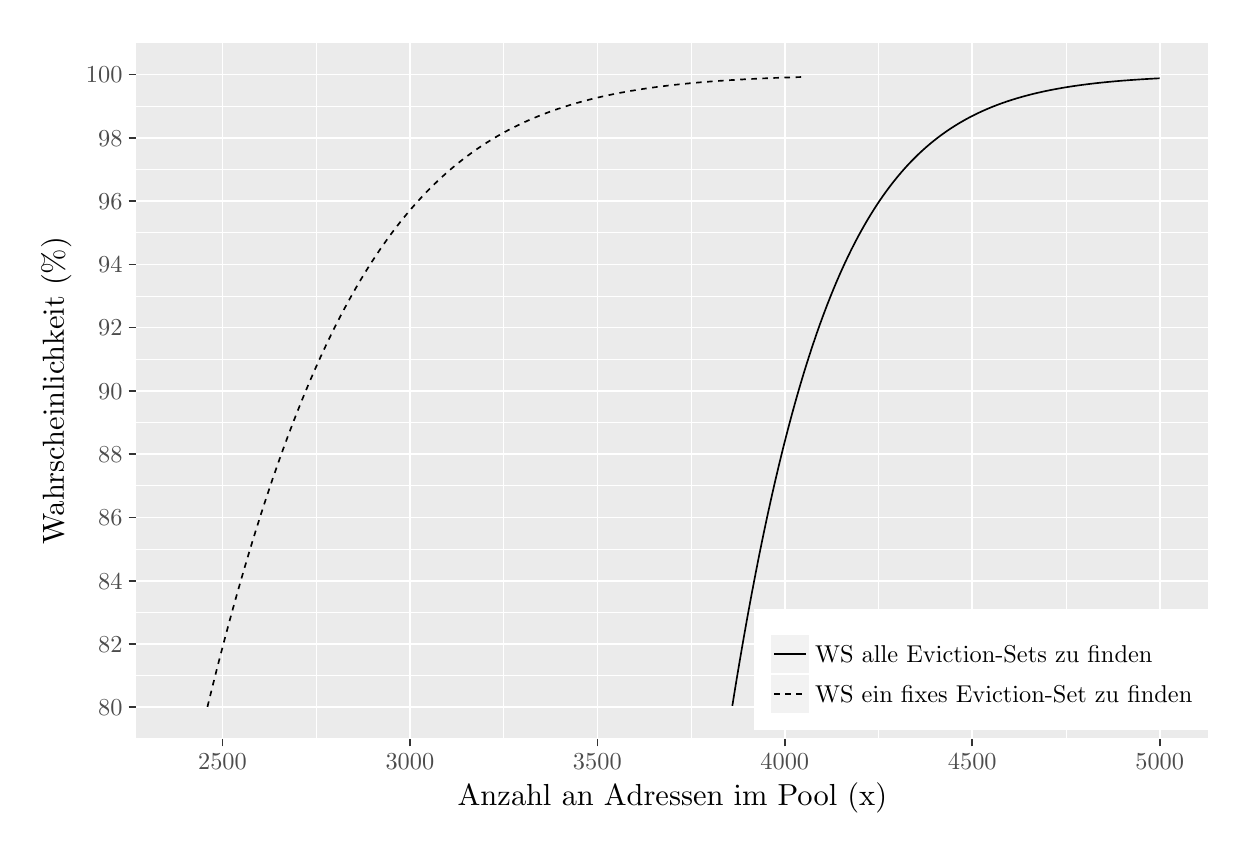
\begin{tikzpicture}[x=1pt,y=1pt]
\definecolor{fillColor}{RGB}{255,255,255}
\path[use as bounding box,fill=fillColor,fill opacity=0.00] (0,0) rectangle (432.17,289.08);
\begin{scope}
\path[clip] (  0.00,  0.00) rectangle (432.17,289.08);
\definecolor{drawColor}{RGB}{255,255,255}
\definecolor{fillColor}{RGB}{255,255,255}

\path[draw=drawColor,line width= 0.6pt,line join=round,line cap=round,fill=fillColor] (  0.00,  0.00) rectangle (432.17,289.08);
\end{scope}
\begin{scope}
\path[clip] ( 39.22, 32.09) rectangle (426.67,283.58);
\definecolor{fillColor}{gray}{0.92}

\path[fill=fillColor] ( 39.22, 32.09) rectangle (426.67,283.58);
\definecolor{drawColor}{RGB}{255,255,255}

\path[draw=drawColor,line width= 0.3pt,line join=round] ( 39.22, 32.09) --
	(426.67, 32.09);

\path[draw=drawColor,line width= 0.3pt,line join=round] ( 39.22, 54.95) --
	(426.67, 54.95);

\path[draw=drawColor,line width= 0.3pt,line join=round] ( 39.22, 77.81) --
	(426.67, 77.81);

\path[draw=drawColor,line width= 0.3pt,line join=round] ( 39.22,100.68) --
	(426.67,100.68);

\path[draw=drawColor,line width= 0.3pt,line join=round] ( 39.22,123.54) --
	(426.67,123.54);

\path[draw=drawColor,line width= 0.3pt,line join=round] ( 39.22,146.40) --
	(426.67,146.40);

\path[draw=drawColor,line width= 0.3pt,line join=round] ( 39.22,169.26) --
	(426.67,169.26);

\path[draw=drawColor,line width= 0.3pt,line join=round] ( 39.22,192.13) --
	(426.67,192.13);

\path[draw=drawColor,line width= 0.3pt,line join=round] ( 39.22,214.99) --
	(426.67,214.99);

\path[draw=drawColor,line width= 0.3pt,line join=round] ( 39.22,237.85) --
	(426.67,237.85);

\path[draw=drawColor,line width= 0.3pt,line join=round] ( 39.22,260.72) --
	(426.67,260.72);

\path[draw=drawColor,line width= 0.3pt,line join=round] ( 39.22,283.58) --
	(426.67,283.58);

\path[draw=drawColor,line width= 0.3pt,line join=round] (104.25, 32.09) --
	(104.25,283.58);

\path[draw=drawColor,line width= 0.3pt,line join=round] (171.99, 32.09) --
	(171.99,283.58);

\path[draw=drawColor,line width= 0.3pt,line join=round] (239.72, 32.09) --
	(239.72,283.58);

\path[draw=drawColor,line width= 0.3pt,line join=round] (307.46, 32.09) --
	(307.46,283.58);

\path[draw=drawColor,line width= 0.3pt,line join=round] (375.19, 32.09) --
	(375.19,283.58);

\path[draw=drawColor,line width= 0.6pt,line join=round] ( 39.22, 43.52) --
	(426.67, 43.52);

\path[draw=drawColor,line width= 0.6pt,line join=round] ( 39.22, 66.38) --
	(426.67, 66.38);

\path[draw=drawColor,line width= 0.6pt,line join=round] ( 39.22, 89.24) --
	(426.67, 89.24);

\path[draw=drawColor,line width= 0.6pt,line join=round] ( 39.22,112.11) --
	(426.67,112.11);

\path[draw=drawColor,line width= 0.6pt,line join=round] ( 39.22,134.97) --
	(426.67,134.97);

\path[draw=drawColor,line width= 0.6pt,line join=round] ( 39.22,157.83) --
	(426.67,157.83);

\path[draw=drawColor,line width= 0.6pt,line join=round] ( 39.22,180.70) --
	(426.67,180.70);

\path[draw=drawColor,line width= 0.6pt,line join=round] ( 39.22,203.56) --
	(426.67,203.56);

\path[draw=drawColor,line width= 0.6pt,line join=round] ( 39.22,226.42) --
	(426.67,226.42);

\path[draw=drawColor,line width= 0.6pt,line join=round] ( 39.22,249.29) --
	(426.67,249.29);

\path[draw=drawColor,line width= 0.6pt,line join=round] ( 39.22,272.15) --
	(426.67,272.15);

\path[draw=drawColor,line width= 0.6pt,line join=round] ( 70.38, 32.09) --
	( 70.38,283.58);

\path[draw=drawColor,line width= 0.6pt,line join=round] (138.12, 32.09) --
	(138.12,283.58);

\path[draw=drawColor,line width= 0.6pt,line join=round] (205.85, 32.09) --
	(205.85,283.58);

\path[draw=drawColor,line width= 0.6pt,line join=round] (273.59, 32.09) --
	(273.59,283.58);

\path[draw=drawColor,line width= 0.6pt,line join=round] (341.33, 32.09) --
	(341.33,283.58);

\path[draw=drawColor,line width= 0.6pt,line join=round] (409.06, 32.09) --
	(409.06,283.58);
\definecolor{drawColor}{RGB}{0,0,0}

\path[draw=drawColor,line width= 0.6pt,line join=round] (254.62, 44.02) --
	(254.76, 44.87) --
	(254.90, 45.71) --
	(255.03, 46.56) --
	(255.17, 47.40) --
	(255.30, 48.23) --
	(255.44, 49.07) --
	(255.57, 49.90) --
	(255.71, 50.73) --
	(255.84, 51.55) --
	(255.98, 52.37) --
	(256.11, 53.20) --
	(256.25, 54.02) --
	(256.39, 54.83) --
	(256.52, 55.64) --
	(256.66, 56.46) --
	(256.79, 57.26) --
	(256.93, 58.07) --
	(257.06, 58.87) --
	(257.20, 59.68) --
	(257.33, 60.47) --
	(257.47, 61.27) --
	(257.60, 62.06) --
	(257.74, 62.85) --
	(257.88, 63.64) --
	(258.01, 64.43) --
	(258.15, 65.21) --
	(258.28, 65.99) --
	(258.42, 66.77) --
	(258.55, 67.55) --
	(258.69, 68.32) --
	(258.82, 69.09) --
	(258.96, 69.86) --
	(259.09, 70.63) --
	(259.23, 71.39) --
	(259.37, 72.16) --
	(259.50, 72.92) --
	(259.64, 73.67) --
	(259.77, 74.43) --
	(259.91, 75.18) --
	(260.04, 75.93) --
	(260.18, 76.68) --
	(260.31, 77.42) --
	(260.45, 78.16) --
	(260.58, 78.90) --
	(260.72, 79.64) --
	(260.86, 80.38) --
	(260.99, 81.11) --
	(261.13, 81.84) --
	(261.26, 82.57) --
	(261.40, 83.29) --
	(261.53, 84.02) --
	(261.67, 84.74) --
	(261.80, 85.46) --
	(261.94, 86.17) --
	(262.08, 86.89) --
	(262.21, 87.60) --
	(262.35, 88.31) --
	(262.48, 89.02) --
	(262.62, 89.72) --
	(262.75, 90.42) --
	(262.89, 91.12) --
	(263.02, 91.82) --
	(263.16, 92.52) --
	(263.29, 93.21) --
	(263.43, 93.90) --
	(263.57, 94.59) --
	(263.70, 95.28) --
	(263.84, 95.96) --
	(263.97, 96.64) --
	(264.11, 97.32) --
	(264.24, 98.00) --
	(264.38, 98.68) --
	(264.51, 99.35) --
	(264.65,100.02) --
	(264.78,100.69) --
	(264.92,101.35) --
	(265.06,102.02) --
	(265.19,102.68) --
	(265.33,103.34) --
	(265.46,104.00) --
	(265.60,104.65) --
	(265.73,105.31) --
	(265.87,105.96) --
	(266.00,106.60) --
	(266.14,107.25) --
	(266.27,107.90) --
	(266.41,108.54) --
	(266.55,109.18) --
	(266.68,109.81) --
	(266.82,110.45) --
	(266.95,111.08) --
	(267.09,111.72) --
	(267.22,112.34) --
	(267.36,112.97) --
	(267.49,113.60) --
	(267.63,114.22) --
	(267.76,114.84) --
	(267.90,115.46) --
	(268.04,116.07) --
	(268.17,116.69) --
	(268.31,117.30) --
	(268.44,117.91) --
	(268.58,118.52) --
	(268.71,119.12) --
	(268.85,119.73) --
	(268.98,120.33) --
	(269.12,120.93) --
	(269.26,121.53) --
	(269.39,122.12) --
	(269.53,122.72) --
	(269.66,123.31) --
	(269.80,123.90) --
	(269.93,124.48) --
	(270.07,125.07) --
	(270.20,125.65) --
	(270.34,126.23) --
	(270.47,126.81) --
	(270.61,127.39) --
	(270.75,127.97) --
	(270.88,128.54) --
	(271.02,129.11) --
	(271.15,129.68) --
	(271.29,130.25) --
	(271.42,130.81) --
	(271.56,131.37) --
	(271.69,131.93) --
	(271.83,132.50) --
	(271.96,133.05) --
	(272.10,133.61) --
	(272.24,134.16) --
	(272.37,134.71) --
	(272.51,135.26) --
	(272.64,135.81) --
	(272.78,136.35) --
	(272.91,136.90) --
	(273.05,137.44) --
	(273.18,137.98) --
	(273.32,138.52) --
	(273.45,139.05) --
	(273.59,139.59) --
	(273.73,140.12) --
	(273.86,140.65) --
	(274.00,141.18) --
	(274.13,141.70) --
	(274.27,142.23) --
	(274.40,142.75) --
	(274.54,143.27) --
	(274.67,143.79) --
	(274.81,144.31) --
	(274.94,144.82) --
	(275.08,145.34) --
	(275.22,145.85) --
	(275.35,146.36) --
	(275.49,146.87) --
	(275.62,147.37) --
	(275.76,147.88) --
	(275.89,148.38) --
	(276.03,148.88) --
	(276.16,149.38) --
	(276.30,149.88) --
	(276.44,150.37) --
	(276.57,150.87) --
	(276.71,151.36) --
	(276.84,151.85) --
	(276.98,152.33) --
	(277.11,152.82) --
	(277.25,153.31) --
	(277.38,153.79) --
	(277.52,154.27) --
	(277.65,154.75) --
	(277.79,155.23) --
	(277.93,155.70) --
	(278.06,156.18) --
	(278.20,156.65) --
	(278.33,157.12) --
	(278.47,157.59) --
	(278.60,158.06) --
	(278.74,158.52) --
	(278.87,158.98) --
	(279.01,159.45) --
	(279.14,159.91) --
	(279.28,160.37) --
	(279.42,160.82) --
	(279.55,161.28) --
	(279.69,161.73) --
	(279.82,162.18) --
	(279.96,162.63) --
	(280.09,163.08) --
	(280.23,163.53) --
	(280.36,163.98) --
	(280.50,164.42) --
	(280.63,164.86) --
	(280.77,165.30) --
	(280.91,165.74) --
	(281.04,166.18) --
	(281.18,166.61) --
	(281.31,167.05) --
	(281.45,167.48) --
	(281.58,167.91) --
	(281.72,168.34) --
	(281.85,168.77) --
	(281.99,169.19) --
	(282.13,169.62) --
	(282.26,170.04) --
	(282.40,170.46) --
	(282.53,170.88) --
	(282.67,171.30) --
	(282.80,171.71) --
	(282.94,172.13) --
	(283.07,172.54) --
	(283.21,172.95) --
	(283.34,173.36) --
	(283.48,173.77) --
	(283.62,174.18) --
	(283.75,174.58) --
	(283.89,174.99) --
	(284.02,175.39) --
	(284.16,175.79) --
	(284.29,176.19) --
	(284.43,176.59) --
	(284.56,176.99) --
	(284.70,177.38) --
	(284.83,177.78) --
	(284.97,178.17) --
	(285.11,178.56) --
	(285.24,178.95) --
	(285.38,179.33) --
	(285.51,179.72) --
	(285.65,180.11) --
	(285.78,180.49) --
	(285.92,180.87) --
	(286.05,181.25) --
	(286.19,181.63) --
	(286.32,182.01) --
	(286.46,182.38) --
	(286.60,182.76) --
	(286.73,183.13) --
	(286.87,183.50) --
	(287.00,183.87) --
	(287.14,184.24) --
	(287.27,184.61) --
	(287.41,184.97) --
	(287.54,185.34) --
	(287.68,185.70) --
	(287.81,186.06) --
	(287.95,186.42) --
	(288.09,186.78) --
	(288.22,187.14) --
	(288.36,187.50) --
	(288.49,187.85) --
	(288.63,188.21) --
	(288.76,188.56) --
	(288.90,188.91) --
	(289.03,189.26) --
	(289.17,189.61) --
	(289.31,189.95) --
	(289.44,190.30) --
	(289.58,190.64) --
	(289.71,190.98) --
	(289.85,191.33) --
	(289.98,191.67) --
	(290.12,192.01) --
	(290.25,192.34) --
	(290.39,192.68) --
	(290.52,193.01) --
	(290.66,193.35) --
	(290.80,193.68) --
	(290.93,194.01) --
	(291.07,194.34) --
	(291.20,194.67) --
	(291.34,195.00) --
	(291.47,195.32) --
	(291.61,195.65) --
	(291.74,195.97) --
	(291.88,196.29) --
	(292.01,196.61) --
	(292.15,196.93) --
	(292.29,197.25) --
	(292.42,197.57) --
	(292.56,197.88) --
	(292.69,198.20) --
	(292.83,198.51) --
	(292.96,198.82) --
	(293.10,199.14) --
	(293.23,199.45) --
	(293.37,199.75) --
	(293.50,200.06) --
	(293.64,200.37) --
	(293.78,200.67) --
	(293.91,200.97) --
	(294.05,201.28) --
	(294.18,201.58) --
	(294.32,201.88) --
	(294.45,202.18) --
	(294.59,202.48) --
	(294.72,202.77) --
	(294.86,203.07) --
	(294.99,203.36) --
	(295.13,203.66) --
	(295.27,203.95) --
	(295.40,204.24) --
	(295.54,204.53) --
	(295.67,204.82) --
	(295.81,205.10) --
	(295.94,205.39) --
	(296.08,205.67) --
	(296.21,205.96) --
	(296.35,206.24) --
	(296.49,206.52) --
	(296.62,206.80) --
	(296.76,207.08) --
	(296.89,207.36) --
	(297.03,207.64) --
	(297.16,207.91) --
	(297.30,208.19) --
	(297.43,208.46) --
	(297.57,208.74) --
	(297.70,209.01) --
	(297.84,209.28) --
	(297.98,209.55) --
	(298.11,209.82) --
	(298.25,210.08) --
	(298.38,210.35) --
	(298.52,210.62) --
	(298.65,210.88) --
	(298.79,211.14) --
	(298.92,211.40) --
	(299.06,211.67) --
	(299.19,211.93) --
	(299.33,212.19) --
	(299.47,212.44) --
	(299.60,212.70) --
	(299.74,212.96) --
	(299.87,213.21) --
	(300.01,213.46) --
	(300.14,213.72) --
	(300.28,213.97) --
	(300.41,214.22) --
	(300.55,214.47) --
	(300.68,214.72) --
	(300.82,214.97) --
	(300.96,215.21) --
	(301.09,215.46) --
	(301.23,215.70) --
	(301.36,215.95) --
	(301.50,216.19) --
	(301.63,216.43) --
	(301.77,216.67) --
	(301.90,216.91) --
	(302.04,217.15) --
	(302.18,217.39) --
	(302.31,217.63) --
	(302.45,217.86) --
	(302.58,218.10) --
	(302.72,218.33) --
	(302.85,218.56) --
	(302.99,218.80) --
	(303.12,219.03) --
	(303.26,219.26) --
	(303.39,219.49) --
	(303.53,219.72) --
	(303.67,219.94) --
	(303.80,220.17) --
	(303.94,220.40) --
	(304.07,220.62) --
	(304.21,220.84) --
	(304.34,221.07) --
	(304.48,221.29) --
	(304.61,221.51) --
	(304.75,221.73) --
	(304.88,221.95) --
	(305.02,222.17) --
	(305.16,222.39) --
	(305.29,222.60) --
	(305.43,222.82) --
	(305.56,223.03) --
	(305.70,223.25) --
	(305.83,223.46) --
	(305.97,223.67) --
	(306.10,223.88) --
	(306.24,224.09) --
	(306.37,224.30) --
	(306.51,224.51) --
	(306.65,224.72) --
	(306.78,224.93) --
	(306.92,225.13) --
	(307.05,225.34) --
	(307.19,225.54) --
	(307.32,225.75) --
	(307.46,225.95) --
	(307.59,226.15) --
	(307.73,226.35) --
	(307.86,226.55) --
	(308.00,226.75) --
	(308.14,226.95) --
	(308.27,227.15) --
	(308.41,227.35) --
	(308.54,227.54) --
	(308.68,227.74) --
	(308.81,227.93) --
	(308.95,228.13) --
	(309.08,228.32) --
	(309.22,228.51) --
	(309.36,228.70) --
	(309.49,228.89) --
	(309.63,229.08) --
	(309.76,229.27) --
	(309.90,229.46) --
	(310.03,229.65) --
	(310.17,229.84) --
	(310.30,230.02) --
	(310.44,230.21) --
	(310.57,230.39) --
	(310.71,230.57) --
	(310.85,230.76) --
	(310.98,230.94) --
	(311.12,231.12) --
	(311.25,231.30) --
	(311.39,231.48) --
	(311.52,231.66) --
	(311.66,231.84) --
	(311.79,232.02) --
	(311.93,232.19) --
	(312.06,232.37) --
	(312.20,232.55) --
	(312.34,232.72) --
	(312.47,232.89) --
	(312.61,233.07) --
	(312.74,233.24) --
	(312.88,233.41) --
	(313.01,233.58) --
	(313.15,233.75) --
	(313.28,233.92) --
	(313.42,234.09) --
	(313.55,234.26) --
	(313.69,234.43) --
	(313.83,234.59) --
	(313.96,234.76) --
	(314.10,234.93) --
	(314.23,235.09) --
	(314.37,235.25) --
	(314.50,235.42) --
	(314.64,235.58) --
	(314.77,235.74) --
	(314.91,235.90) --
	(315.04,236.06) --
	(315.18,236.22) --
	(315.32,236.38) --
	(315.45,236.54) --
	(315.59,236.70) --
	(315.72,236.86) --
	(315.86,237.01) --
	(315.99,237.17) --
	(316.13,237.32) --
	(316.26,237.48) --
	(316.40,237.63) --
	(316.54,237.79) --
	(316.67,237.94) --
	(316.81,238.09) --
	(316.94,238.24) --
	(317.08,238.39) --
	(317.21,238.54) --
	(317.35,238.69) --
	(317.48,238.84) --
	(317.62,238.99) --
	(317.75,239.14) --
	(317.89,239.29) --
	(318.03,239.43) --
	(318.16,239.58) --
	(318.30,239.72) --
	(318.43,239.87) --
	(318.57,240.01) --
	(318.70,240.15) --
	(318.84,240.30) --
	(318.97,240.44) --
	(319.11,240.58) --
	(319.24,240.72) --
	(319.38,240.86) --
	(319.52,241.00) --
	(319.65,241.14) --
	(319.79,241.28) --
	(319.92,241.42) --
	(320.06,241.55) --
	(320.19,241.69) --
	(320.33,241.83) --
	(320.46,241.96) --
	(320.60,242.10) --
	(320.73,242.23) --
	(320.87,242.36) --
	(321.01,242.50) --
	(321.14,242.63) --
	(321.28,242.76) --
	(321.41,242.90) --
	(321.55,243.03) --
	(321.68,243.16) --
	(321.82,243.29) --
	(321.95,243.42) --
	(322.09,243.54) --
	(322.23,243.67) --
	(322.36,243.80) --
	(322.50,243.93) --
	(322.63,244.05) --
	(322.77,244.18) --
	(322.90,244.31) --
	(323.04,244.43) --
	(323.17,244.56) --
	(323.31,244.68) --
	(323.44,244.80) --
	(323.58,244.93) --
	(323.72,245.05) --
	(323.85,245.17) --
	(323.99,245.29) --
	(324.12,245.41) --
	(324.26,245.53) --
	(324.39,245.65) --
	(324.53,245.77) --
	(324.66,245.89) --
	(324.80,246.01) --
	(324.93,246.13) --
	(325.07,246.24) --
	(325.21,246.36) --
	(325.34,246.48) --
	(325.48,246.59) --
	(325.61,246.71) --
	(325.75,246.82) --
	(325.88,246.94) --
	(326.02,247.05) --
	(326.15,247.16) --
	(326.29,247.27) --
	(326.42,247.39) --
	(326.56,247.50) --
	(326.70,247.61) --
	(326.83,247.72) --
	(326.97,247.83) --
	(327.10,247.94) --
	(327.24,248.05) --
	(327.37,248.16) --
	(327.51,248.27) --
	(327.64,248.38) --
	(327.78,248.48) --
	(327.91,248.59) --
	(328.05,248.70) --
	(328.19,248.80) --
	(328.32,248.91) --
	(328.46,249.01) --
	(328.59,249.12) --
	(328.73,249.22) --
	(328.86,249.33) --
	(329.00,249.43) --
	(329.13,249.53) --
	(329.27,249.64) --
	(329.41,249.74) --
	(329.54,249.84) --
	(329.68,249.94) --
	(329.81,250.04) --
	(329.95,250.14) --
	(330.08,250.24) --
	(330.22,250.34) --
	(330.35,250.44) --
	(330.49,250.54) --
	(330.62,250.64) --
	(330.76,250.73) --
	(330.90,250.83) --
	(331.03,250.93) --
	(331.17,251.02) --
	(331.30,251.12) --
	(331.44,251.22) --
	(331.57,251.31) --
	(331.71,251.41) --
	(331.84,251.50) --
	(331.98,251.59) --
	(332.11,251.69) --
	(332.25,251.78) --
	(332.39,251.87) --
	(332.52,251.96) --
	(332.66,252.06) --
	(332.79,252.15) --
	(332.93,252.24) --
	(333.06,252.33) --
	(333.20,252.42) --
	(333.33,252.51) --
	(333.47,252.60) --
	(333.60,252.69) --
	(333.74,252.78) --
	(333.88,252.87) --
	(334.01,252.95) --
	(334.15,253.04) --
	(334.28,253.13) --
	(334.42,253.22) --
	(334.55,253.30) --
	(334.69,253.39) --
	(334.82,253.47) --
	(334.96,253.56) --
	(335.09,253.64) --
	(335.23,253.73) --
	(335.37,253.81) --
	(335.50,253.90) --
	(335.64,253.98) --
	(335.77,254.06) --
	(335.91,254.15) --
	(336.04,254.23) --
	(336.18,254.31) --
	(336.31,254.39) --
	(336.45,254.47) --
	(336.59,254.55) --
	(336.72,254.64) --
	(336.86,254.72) --
	(336.99,254.80) --
	(337.13,254.87) --
	(337.26,254.95) --
	(337.40,255.03) --
	(337.53,255.11) --
	(337.67,255.19) --
	(337.80,255.27) --
	(337.94,255.34) --
	(338.08,255.42) --
	(338.21,255.50) --
	(338.35,255.57) --
	(338.48,255.65) --
	(338.62,255.73) --
	(338.75,255.80) --
	(338.89,255.88) --
	(339.02,255.95) --
	(339.16,256.03) --
	(339.29,256.10) --
	(339.43,256.17) --
	(339.57,256.25) --
	(339.70,256.32) --
	(339.84,256.39) --
	(339.97,256.47) --
	(340.11,256.54) --
	(340.24,256.61) --
	(340.38,256.68) --
	(340.51,256.75) --
	(340.65,256.82) --
	(340.78,256.89) --
	(340.92,256.96) --
	(341.06,257.03) --
	(341.19,257.10) --
	(341.33,257.17) --
	(341.46,257.24) --
	(341.60,257.31) --
	(341.73,257.38) --
	(341.87,257.45) --
	(342.00,257.51) --
	(342.14,257.58) --
	(342.28,257.65) --
	(342.41,257.72) --
	(342.55,257.78) --
	(342.68,257.85) --
	(342.82,257.92) --
	(342.95,257.98) --
	(343.09,258.05) --
	(343.22,258.11) --
	(343.36,258.18) --
	(343.49,258.24) --
	(343.63,258.30) --
	(343.77,258.37) --
	(343.90,258.43) --
	(344.04,258.50) --
	(344.17,258.56) --
	(344.31,258.62) --
	(344.44,258.68) --
	(344.58,258.75) --
	(344.71,258.81) --
	(344.85,258.87) --
	(344.98,258.93) --
	(345.12,258.99) --
	(345.26,259.05) --
	(345.39,259.11) --
	(345.53,259.17) --
	(345.66,259.23) --
	(345.80,259.29) --
	(345.93,259.35) --
	(346.07,259.41) --
	(346.20,259.47) --
	(346.34,259.53) --
	(346.47,259.59) --
	(346.61,259.65) --
	(346.75,259.71) --
	(346.88,259.76) --
	(347.02,259.82) --
	(347.15,259.88) --
	(347.29,259.94) --
	(347.42,259.99) --
	(347.56,260.05) --
	(347.69,260.10) --
	(347.83,260.16) --
	(347.96,260.22) --
	(348.10,260.27) --
	(348.24,260.33) --
	(348.37,260.38) --
	(348.51,260.44) --
	(348.64,260.49) --
	(348.78,260.54) --
	(348.91,260.60) --
	(349.05,260.65) --
	(349.18,260.71) --
	(349.32,260.76) --
	(349.46,260.81) --
	(349.59,260.86) --
	(349.73,260.92) --
	(349.86,260.97) --
	(350.00,261.02) --
	(350.13,261.07) --
	(350.27,261.13) --
	(350.40,261.18) --
	(350.54,261.23) --
	(350.67,261.28) --
	(350.81,261.33) --
	(350.95,261.38) --
	(351.08,261.43) --
	(351.22,261.48) --
	(351.35,261.53) --
	(351.49,261.58) --
	(351.62,261.63) --
	(351.76,261.68) --
	(351.89,261.73) --
	(352.03,261.77) --
	(352.16,261.82) --
	(352.30,261.87) --
	(352.44,261.92) --
	(352.57,261.97) --
	(352.71,262.01) --
	(352.84,262.06) --
	(352.98,262.11) --
	(353.11,262.16) --
	(353.25,262.20) --
	(353.38,262.25) --
	(353.52,262.30) --
	(353.65,262.34) --
	(353.79,262.39) --
	(353.93,262.43) --
	(354.06,262.48) --
	(354.20,262.52) --
	(354.33,262.57) --
	(354.47,262.61) --
	(354.60,262.66) --
	(354.74,262.70) --
	(354.87,262.75) --
	(355.01,262.79) --
	(355.14,262.84) --
	(355.28,262.88) --
	(355.42,262.92) --
	(355.55,262.97) --
	(355.69,263.01) --
	(355.82,263.05) --
	(355.96,263.09) --
	(356.09,263.14) --
	(356.23,263.18) --
	(356.36,263.22) --
	(356.50,263.26) --
	(356.64,263.30) --
	(356.77,263.35) --
	(356.91,263.39) --
	(357.04,263.43) --
	(357.18,263.47) --
	(357.31,263.51) --
	(357.45,263.55) --
	(357.58,263.59) --
	(357.72,263.63) --
	(357.85,263.67) --
	(357.99,263.71) --
	(358.13,263.75) --
	(358.26,263.79) --
	(358.40,263.83) --
	(358.53,263.87) --
	(358.67,263.91) --
	(358.80,263.95) --
	(358.94,263.98) --
	(359.07,264.02) --
	(359.21,264.06) --
	(359.34,264.10) --
	(359.48,264.14) --
	(359.62,264.17) --
	(359.75,264.21) --
	(359.89,264.25) --
	(360.02,264.29) --
	(360.16,264.32) --
	(360.29,264.36) --
	(360.43,264.40) --
	(360.56,264.43) --
	(360.70,264.47) --
	(360.83,264.51) --
	(360.97,264.54) --
	(361.11,264.58) --
	(361.24,264.61) --
	(361.38,264.65) --
	(361.51,264.68) --
	(361.65,264.72) --
	(361.78,264.75) --
	(361.92,264.79) --
	(362.05,264.82) --
	(362.19,264.86) --
	(362.32,264.89) --
	(362.46,264.93) --
	(362.60,264.96) --
	(362.73,265.00) --
	(362.87,265.03) --
	(363.00,265.06) --
	(363.14,265.10) --
	(363.27,265.13) --
	(363.41,265.16) --
	(363.54,265.20) --
	(363.68,265.23) --
	(363.82,265.26) --
	(363.95,265.29) --
	(364.09,265.33) --
	(364.22,265.36) --
	(364.36,265.39) --
	(364.49,265.42) --
	(364.63,265.46) --
	(364.76,265.49) --
	(364.90,265.52) --
	(365.03,265.55) --
	(365.17,265.58) --
	(365.31,265.61) --
	(365.44,265.64) --
	(365.58,265.67) --
	(365.71,265.70) --
	(365.85,265.74) --
	(365.98,265.77) --
	(366.12,265.80) --
	(366.25,265.83) --
	(366.39,265.86) --
	(366.52,265.89) --
	(366.66,265.91) --
	(366.80,265.94) --
	(366.93,265.97) --
	(367.07,266.00) --
	(367.20,266.03) --
	(367.34,266.06) --
	(367.47,266.09) --
	(367.61,266.12) --
	(367.74,266.15) --
	(367.88,266.18) --
	(368.01,266.21) --
	(368.15,266.23) --
	(368.29,266.26) --
	(368.42,266.29) --
	(368.56,266.32) --
	(368.69,266.34) --
	(368.83,266.37) --
	(368.96,266.40) --
	(369.10,266.43) --
	(369.23,266.45) --
	(369.37,266.48) --
	(369.51,266.51) --
	(369.64,266.54) --
	(369.78,266.56) --
	(369.91,266.59) --
	(370.05,266.62) --
	(370.18,266.64) --
	(370.32,266.67) --
	(370.45,266.69) --
	(370.59,266.72) --
	(370.72,266.75) --
	(370.86,266.77) --
	(371.00,266.80) --
	(371.13,266.82) --
	(371.27,266.85) --
	(371.40,266.87) --
	(371.54,266.90) --
	(371.67,266.92) --
	(371.81,266.95) --
	(371.94,266.97) --
	(372.08,267.00) --
	(372.21,267.02) --
	(372.35,267.05) --
	(372.49,267.07) --
	(372.62,267.10) --
	(372.76,267.12) --
	(372.89,267.14) --
	(373.03,267.17) --
	(373.16,267.19) --
	(373.30,267.21) --
	(373.43,267.24) --
	(373.57,267.26) --
	(373.70,267.29) --
	(373.84,267.31) --
	(373.98,267.33) --
	(374.11,267.35) --
	(374.25,267.38) --
	(374.38,267.40) --
	(374.52,267.42) --
	(374.65,267.45) --
	(374.79,267.47) --
	(374.92,267.49) --
	(375.06,267.51) --
	(375.19,267.53) --
	(375.33,267.56) --
	(375.47,267.58) --
	(375.60,267.60) --
	(375.74,267.62) --
	(375.87,267.64) --
	(376.01,267.67) --
	(376.14,267.69) --
	(376.28,267.71) --
	(376.41,267.73) --
	(376.55,267.75) --
	(376.69,267.77) --
	(376.82,267.79) --
	(376.96,267.81) --
	(377.09,267.83) --
	(377.23,267.85) --
	(377.36,267.88) --
	(377.50,267.90) --
	(377.63,267.92) --
	(377.77,267.94) --
	(377.90,267.96) --
	(378.04,267.98) --
	(378.18,268.00) --
	(378.31,268.02) --
	(378.45,268.04) --
	(378.58,268.06) --
	(378.72,268.08) --
	(378.85,268.10) --
	(378.99,268.12) --
	(379.12,268.13) --
	(379.26,268.15) --
	(379.39,268.17) --
	(379.53,268.19) --
	(379.67,268.21) --
	(379.80,268.23) --
	(379.94,268.25) --
	(380.07,268.27) --
	(380.21,268.29) --
	(380.34,268.31) --
	(380.48,268.32) --
	(380.61,268.34) --
	(380.75,268.36) --
	(380.88,268.38) --
	(381.02,268.40) --
	(381.16,268.41) --
	(381.29,268.43) --
	(381.43,268.45) --
	(381.56,268.47) --
	(381.70,268.49) --
	(381.83,268.50) --
	(381.97,268.52) --
	(382.10,268.54) --
	(382.24,268.56) --
	(382.37,268.57) --
	(382.51,268.59) --
	(382.65,268.61) --
	(382.78,268.63) --
	(382.92,268.64) --
	(383.05,268.66) --
	(383.19,268.68) --
	(383.32,268.69) --
	(383.46,268.71) --
	(383.59,268.73) --
	(383.73,268.74) --
	(383.87,268.76) --
	(384.00,268.78) --
	(384.14,268.79) --
	(384.27,268.81) --
	(384.41,268.82) --
	(384.54,268.84) --
	(384.68,268.86) --
	(384.81,268.87) --
	(384.95,268.89) --
	(385.08,268.90) --
	(385.22,268.92) --
	(385.36,268.93) --
	(385.49,268.95) --
	(385.63,268.97) --
	(385.76,268.98) --
	(385.90,269.00) --
	(386.03,269.01) --
	(386.17,269.03) --
	(386.30,269.04) --
	(386.44,269.06) --
	(386.57,269.07) --
	(386.71,269.09) --
	(386.85,269.10) --
	(386.98,269.12) --
	(387.12,269.13) --
	(387.25,269.15) --
	(387.39,269.16) --
	(387.52,269.17) --
	(387.66,269.19) --
	(387.79,269.20) --
	(387.93,269.22) --
	(388.06,269.23) --
	(388.20,269.25) --
	(388.34,269.26) --
	(388.47,269.27) --
	(388.61,269.29) --
	(388.74,269.30) --
	(388.88,269.32) --
	(389.01,269.33) --
	(389.15,269.34) --
	(389.28,269.36) --
	(389.42,269.37) --
	(389.56,269.38) --
	(389.69,269.40) --
	(389.83,269.41) --
	(389.96,269.42) --
	(390.10,269.44) --
	(390.23,269.45) --
	(390.37,269.46) --
	(390.50,269.48) --
	(390.64,269.49) --
	(390.77,269.50) --
	(390.91,269.51) --
	(391.05,269.53) --
	(391.18,269.54) --
	(391.32,269.55) --
	(391.45,269.56) --
	(391.59,269.58) --
	(391.72,269.59) --
	(391.86,269.60) --
	(391.99,269.62) --
	(392.13,269.63) --
	(392.26,269.64) --
	(392.40,269.65) --
	(392.54,269.66) --
	(392.67,269.68) --
	(392.81,269.69) --
	(392.94,269.70) --
	(393.08,269.71) --
	(393.21,269.72) --
	(393.35,269.74) --
	(393.48,269.75) --
	(393.62,269.76) --
	(393.75,269.77) --
	(393.89,269.78) --
	(394.03,269.79) --
	(394.16,269.80) --
	(394.30,269.82) --
	(394.43,269.83) --
	(394.57,269.84) --
	(394.70,269.85) --
	(394.84,269.86) --
	(394.97,269.87) --
	(395.11,269.88) --
	(395.24,269.90) --
	(395.38,269.91) --
	(395.52,269.92) --
	(395.65,269.93) --
	(395.79,269.94) --
	(395.92,269.95) --
	(396.06,269.96) --
	(396.19,269.97) --
	(396.33,269.98) --
	(396.46,269.99) --
	(396.60,270.00) --
	(396.74,270.01) --
	(396.87,270.02) --
	(397.01,270.03) --
	(397.14,270.04) --
	(397.28,270.05) --
	(397.41,270.06) --
	(397.55,270.07) --
	(397.68,270.09) --
	(397.82,270.10) --
	(397.95,270.11) --
	(398.09,270.12) --
	(398.23,270.13) --
	(398.36,270.14) --
	(398.50,270.14) --
	(398.63,270.15) --
	(398.77,270.17) --
	(398.90,270.17) --
	(399.04,270.18) --
	(399.17,270.19) --
	(399.31,270.20) --
	(399.44,270.21) --
	(399.58,270.22) --
	(399.72,270.23) --
	(399.85,270.24) --
	(399.99,270.25) --
	(400.12,270.26) --
	(400.26,270.27) --
	(400.39,270.28) --
	(400.53,270.29) --
	(400.66,270.30) --
	(400.80,270.31) --
	(400.93,270.31) --
	(401.07,270.32) --
	(401.21,270.33) --
	(401.34,270.34) --
	(401.48,270.35) --
	(401.61,270.36) --
	(401.75,270.37) --
	(401.88,270.38) --
	(402.02,270.38) --
	(402.15,270.39) --
	(402.29,270.40) --
	(402.42,270.41) --
	(402.56,270.42) --
	(402.70,270.43) --
	(402.83,270.44) --
	(402.97,270.45) --
	(403.10,270.45) --
	(403.24,270.46) --
	(403.37,270.47) --
	(403.51,270.48) --
	(403.64,270.49) --
	(403.78,270.49) --
	(403.92,270.50) --
	(404.05,270.51) --
	(404.19,270.52) --
	(404.32,270.53) --
	(404.46,270.53) --
	(404.59,270.54) --
	(404.73,270.55) --
	(404.86,270.56) --
	(405.00,270.57) --
	(405.13,270.57) --
	(405.27,270.58) --
	(405.41,270.59) --
	(405.54,270.60) --
	(405.68,270.61) --
	(405.81,270.61) --
	(405.95,270.62) --
	(406.08,270.63) --
	(406.22,270.63) --
	(406.35,270.64) --
	(406.49,270.65) --
	(406.62,270.66) --
	(406.76,270.66) --
	(406.90,270.67) --
	(407.03,270.68) --
	(407.17,270.69) --
	(407.30,270.69) --
	(407.44,270.70) --
	(407.57,270.71) --
	(407.71,270.71) --
	(407.84,270.72) --
	(407.98,270.73) --
	(408.11,270.74) --
	(408.25,270.74) --
	(408.39,270.75) --
	(408.52,270.76) --
	(408.66,270.76) --
	(408.79,270.77) --
	(408.93,270.78) --
	(409.06,270.78);

\path[draw=drawColor,line width= 0.6pt,dash pattern=on 2pt off 2pt ,line join=round] ( 64.96, 43.67) --
	( 65.10, 44.22) --
	( 65.23, 44.78) --
	( 65.37, 45.33) --
	( 65.50, 45.88) --
	( 65.64, 46.43) --
	( 65.77, 46.98) --
	( 65.91, 47.53) --
	( 66.05, 48.07) --
	( 66.18, 48.62) --
	( 66.32, 49.17) --
	( 66.45, 49.71) --
	( 66.59, 50.25) --
	( 66.72, 50.80) --
	( 66.86, 51.34) --
	( 66.99, 51.88) --
	( 67.13, 52.42) --
	( 67.27, 52.96) --
	( 67.40, 53.49) --
	( 67.54, 54.03) --
	( 67.67, 54.57) --
	( 67.81, 55.10) --
	( 67.94, 55.64) --
	( 68.08, 56.17) --
	( 68.21, 56.70) --
	( 68.35, 57.24) --
	( 68.48, 57.76) --
	( 68.62, 58.29) --
	( 68.76, 58.82) --
	( 68.89, 59.34) --
	( 69.03, 59.87) --
	( 69.16, 60.40) --
	( 69.30, 60.92) --
	( 69.43, 61.44) --
	( 69.57, 61.97) --
	( 69.70, 62.49) --
	( 69.84, 63.01) --
	( 69.97, 63.53) --
	( 70.11, 64.05) --
	( 70.25, 64.57) --
	( 70.38, 65.09) --
	( 70.52, 65.59) --
	( 70.65, 66.11) --
	( 70.79, 66.63) --
	( 70.92, 67.14) --
	( 71.06, 67.65) --
	( 71.19, 68.17) --
	( 71.33, 68.68) --
	( 71.46, 69.19) --
	( 71.60, 69.69) --
	( 71.74, 70.20) --
	( 71.87, 70.70) --
	( 72.01, 71.21) --
	( 72.14, 71.71) --
	( 72.28, 72.22) --
	( 72.41, 72.72) --
	( 72.55, 73.22) --
	( 72.68, 73.72) --
	( 72.82, 74.22) --
	( 72.95, 74.72) --
	( 73.09, 75.22) --
	( 73.23, 75.72) --
	( 73.36, 76.21) --
	( 73.50, 76.71) --
	( 73.63, 77.20) --
	( 73.77, 77.70) --
	( 73.90, 78.19) --
	( 74.04, 78.68) --
	( 74.17, 79.17) --
	( 74.31, 79.66) --
	( 74.45, 80.15) --
	( 74.58, 80.64) --
	( 74.72, 81.13) --
	( 74.85, 81.61) --
	( 74.99, 82.10) --
	( 75.12, 82.58) --
	( 75.26, 83.06) --
	( 75.39, 83.55) --
	( 75.53, 84.03) --
	( 75.66, 84.51) --
	( 75.80, 84.98) --
	( 75.94, 85.47) --
	( 76.07, 85.95) --
	( 76.21, 86.42) --
	( 76.34, 86.90) --
	( 76.48, 87.37) --
	( 76.61, 87.84) --
	( 76.75, 88.32) --
	( 76.88, 88.79) --
	( 77.02, 89.26) --
	( 77.15, 89.74) --
	( 77.29, 90.20) --
	( 77.43, 90.67) --
	( 77.56, 91.14) --
	( 77.70, 91.60) --
	( 77.83, 92.07) --
	( 77.97, 92.54) --
	( 78.10, 93.00) --
	( 78.24, 93.46) --
	( 78.37, 93.92) --
	( 78.51, 94.39) --
	( 78.64, 94.84) --
	( 78.78, 95.31) --
	( 78.92, 95.76) --
	( 79.05, 96.22) --
	( 79.19, 96.68) --
	( 79.32, 97.14) --
	( 79.46, 97.59) --
	( 79.59, 98.04) --
	( 79.73, 98.50) --
	( 79.86, 98.95) --
	( 80.00, 99.40) --
	( 80.13, 99.85) --
	( 80.27,100.30) --
	( 80.41,100.75) --
	( 80.54,101.19) --
	( 80.68,101.64) --
	( 80.81,102.09) --
	( 80.95,102.53) --
	( 81.08,102.98) --
	( 81.22,103.43) --
	( 81.35,103.86) --
	( 81.49,104.31) --
	( 81.63,104.75) --
	( 81.76,105.19) --
	( 81.90,105.62) --
	( 82.03,106.06) --
	( 82.17,106.50) --
	( 82.30,106.94) --
	( 82.44,107.37) --
	( 82.57,107.80) --
	( 82.71,108.24) --
	( 82.84,108.67) --
	( 82.98,109.11) --
	( 83.12,109.53) --
	( 83.25,109.96) --
	( 83.39,110.39) --
	( 83.52,110.82) --
	( 83.66,111.25) --
	( 83.79,111.68) --
	( 83.93,112.10) --
	( 84.06,112.53) --
	( 84.20,112.95) --
	( 84.33,113.38) --
	( 84.47,113.79) --
	( 84.61,114.21) --
	( 84.74,114.63) --
	( 84.88,115.05) --
	( 85.01,115.47) --
	( 85.15,115.89) --
	( 85.28,116.31) --
	( 85.42,116.72) --
	( 85.55,117.14) --
	( 85.69,117.55) --
	( 85.82,117.97) --
	( 85.96,118.39) --
	( 86.10,118.80) --
	( 86.23,119.21) --
	( 86.37,119.62) --
	( 86.50,120.02) --
	( 86.64,120.43) --
	( 86.77,120.84) --
	( 86.91,121.24) --
	( 87.04,121.65) --
	( 87.18,122.06) --
	( 87.32,122.46) --
	( 87.45,122.86) --
	( 87.59,123.26) --
	( 87.72,123.66) --
	( 87.86,124.07) --
	( 87.99,124.47) --
	( 88.13,124.87) --
	( 88.26,125.26) --
	( 88.40,125.66) --
	( 88.53,126.06) --
	( 88.67,126.45) --
	( 88.81,126.85) --
	( 88.94,127.24) --
	( 89.08,127.64) --
	( 89.21,128.03) --
	( 89.35,128.41) --
	( 89.48,128.81) --
	( 89.62,129.20) --
	( 89.75,129.58) --
	( 89.89,129.98) --
	( 90.02,130.36) --
	( 90.16,130.75) --
	( 90.30,131.14) --
	( 90.43,131.52) --
	( 90.57,131.91) --
	( 90.70,132.28) --
	( 90.84,132.67) --
	( 90.97,133.05) --
	( 91.11,133.43) --
	( 91.24,133.81) --
	( 91.38,134.18) --
	( 91.51,134.57) --
	( 91.65,134.94) --
	( 91.79,135.32) --
	( 91.92,135.69) --
	( 92.06,136.07) --
	( 92.19,136.44) --
	( 92.33,136.82) --
	( 92.46,137.19) --
	( 92.60,137.56) --
	( 92.73,137.94) --
	( 92.87,138.30) --
	( 93.00,138.67) --
	( 93.14,139.04) --
	( 93.28,139.41) --
	( 93.41,139.77) --
	( 93.55,140.14) --
	( 93.68,140.51) --
	( 93.82,140.86) --
	( 93.95,141.23) --
	( 94.09,141.60) --
	( 94.22,141.95) --
	( 94.36,142.32) --
	( 94.50,142.68) --
	( 94.63,143.03) --
	( 94.77,143.39) --
	( 94.90,143.75) --
	( 95.04,144.11) --
	( 95.17,144.46) --
	( 95.31,144.82) --
	( 95.44,145.18) --
	( 95.58,145.53) --
	( 95.71,145.88) --
	( 95.85,146.23) --
	( 95.99,146.59) --
	( 96.12,146.94) --
	( 96.26,147.29) --
	( 96.39,147.63) --
	( 96.53,147.98) --
	( 96.66,148.33) --
	( 96.80,148.68) --
	( 96.93,149.03) --
	( 97.07,149.37) --
	( 97.20,149.71) --
	( 97.34,150.05) --
	( 97.48,150.40) --
	( 97.61,150.74) --
	( 97.75,151.08) --
	( 97.88,151.42) --
	( 98.02,151.76) --
	( 98.15,152.10) --
	( 98.29,152.44) --
	( 98.42,152.78) --
	( 98.56,153.11) --
	( 98.69,153.45) --
	( 98.83,153.79) --
	( 98.97,154.12) --
	( 99.10,154.45) --
	( 99.24,154.79) --
	( 99.37,155.12) --
	( 99.51,155.45) --
	( 99.64,155.78) --
	( 99.78,156.11) --
	( 99.91,156.44) --
	(100.05,156.76) --
	(100.18,157.09) --
	(100.32,157.42) --
	(100.46,157.74) --
	(100.59,158.07) --
	(100.73,158.40) --
	(100.86,158.72) --
	(101.00,159.04) --
	(101.13,159.36) --
	(101.27,159.68) --
	(101.40,160.00) --
	(101.54,160.32) --
	(101.68,160.65) --
	(101.81,160.96) --
	(101.95,161.28) --
	(102.08,161.59) --
	(102.22,161.91) --
	(102.35,162.23) --
	(102.49,162.54) --
	(102.62,162.86) --
	(102.76,163.17) --
	(102.89,163.49) --
	(103.03,163.79) --
	(103.17,164.10) --
	(103.30,164.42) --
	(103.44,164.73) --
	(103.57,165.03) --
	(103.71,165.34) --
	(103.84,165.65) --
	(103.98,165.96) --
	(104.11,166.26) --
	(104.25,166.57) --
	(104.38,166.87) --
	(104.52,167.17) --
	(104.66,167.48) --
	(104.79,167.78) --
	(104.93,168.09) --
	(105.06,168.38) --
	(105.20,168.68) --
	(105.33,168.98) --
	(105.47,169.28) --
	(105.60,169.58) --
	(105.74,169.88) --
	(105.87,170.18) --
	(106.01,170.47) --
	(106.15,170.76) --
	(106.28,171.06) --
	(106.42,171.35) --
	(106.55,171.65) --
	(106.69,171.93) --
	(106.82,172.23) --
	(106.96,172.52) --
	(107.09,172.81) --
	(107.23,173.10) --
	(107.37,173.39) --
	(107.50,173.68) --
	(107.64,173.96) --
	(107.77,174.25) --
	(107.91,174.53) --
	(108.04,174.82) --
	(108.18,175.11) --
	(108.31,175.39) --
	(108.45,175.68) --
	(108.58,175.95) --
	(108.72,176.24) --
	(108.86,176.52) --
	(108.99,176.80) --
	(109.13,177.08) --
	(109.26,177.36) --
	(109.40,177.64) --
	(109.53,177.92) --
	(109.67,178.20) --
	(109.80,178.47) --
	(109.94,178.75) --
	(110.07,179.02) --
	(110.21,179.29) --
	(110.35,179.57) --
	(110.48,179.84) --
	(110.62,180.12) --
	(110.75,180.38) --
	(110.89,180.66) --
	(111.02,180.93) --
	(111.16,181.20) --
	(111.29,181.46) --
	(111.43,181.73) --
	(111.56,182.00) --
	(111.70,182.27) --
	(111.84,182.54) --
	(111.97,182.80) --
	(112.11,183.06) --
	(112.24,183.33) --
	(112.38,183.60) --
	(112.51,183.86) --
	(112.65,184.12) --
	(112.78,184.38) --
	(112.92,184.64) --
	(113.05,184.90) --
	(113.19,185.16) --
	(113.33,185.42) --
	(113.46,185.68) --
	(113.60,185.94) --
	(113.73,186.20) --
	(113.87,186.46) --
	(114.00,186.71) --
	(114.14,186.97) --
	(114.27,187.22) --
	(114.41,187.47) --
	(114.55,187.72) --
	(114.68,187.97) --
	(114.82,188.23) --
	(114.95,188.48) --
	(115.09,188.73) --
	(115.22,188.98) --
	(115.36,189.23) --
	(115.49,189.48) --
	(115.63,189.73) --
	(115.76,189.98) --
	(115.90,190.23) --
	(116.04,190.48) --
	(116.17,190.72) --
	(116.31,190.97) --
	(116.44,191.21) --
	(116.58,191.45) --
	(116.71,191.69) --
	(116.85,191.94) --
	(116.98,192.18) --
	(117.12,192.42) --
	(117.25,192.66) --
	(117.39,192.90) --
	(117.53,193.14) --
	(117.66,193.38) --
	(117.80,193.62) --
	(117.93,193.86) --
	(118.07,194.09) --
	(118.20,194.33) --
	(118.34,194.57) --
	(118.47,194.80) --
	(118.61,195.04) --
	(118.74,195.27) --
	(118.88,195.50) --
	(119.02,195.74) --
	(119.15,195.97) --
	(119.29,196.20) --
	(119.42,196.43) --
	(119.56,196.66) --
	(119.69,196.90) --
	(119.83,197.12) --
	(119.96,197.35) --
	(120.10,197.58) --
	(120.23,197.81) --
	(120.37,198.03) --
	(120.51,198.26) --
	(120.64,198.49) --
	(120.78,198.71) --
	(120.91,198.93) --
	(121.05,199.16) --
	(121.18,199.38) --
	(121.32,199.60) --
	(121.45,199.83) --
	(121.59,200.05) --
	(121.73,200.27) --
	(121.86,200.49) --
	(122.00,200.71) --
	(122.13,200.93) --
	(122.27,201.15) --
	(122.40,201.37) --
	(122.54,201.59) --
	(122.67,201.80) --
	(122.81,202.02) --
	(122.94,202.24) --
	(123.08,202.45) --
	(123.22,202.67) --
	(123.35,202.88) --
	(123.49,203.09) --
	(123.62,203.31) --
	(123.76,203.51) --
	(123.89,203.73) --
	(124.03,203.94) --
	(124.16,204.16) --
	(124.30,204.36) --
	(124.43,204.58) --
	(124.57,204.78) --
	(124.71,204.99) --
	(124.84,205.20) --
	(124.98,205.41) --
	(125.11,205.61) --
	(125.25,205.82) --
	(125.38,206.02) --
	(125.52,206.23) --
	(125.65,206.43) --
	(125.79,206.64) --
	(125.92,206.85) --
	(126.06,207.05) --
	(126.20,207.25) --
	(126.33,207.45) --
	(126.47,207.65) --
	(126.60,207.85) --
	(126.74,208.05) --
	(126.87,208.26) --
	(127.01,208.45) --
	(127.14,208.65) --
	(127.28,208.86) --
	(127.42,209.05) --
	(127.55,209.25) --
	(127.69,209.44) --
	(127.82,209.64) --
	(127.96,209.84) --
	(128.09,210.03) --
	(128.23,210.22) --
	(128.36,210.42) --
	(128.50,210.61) --
	(128.63,210.80) --
	(128.77,211.00) --
	(128.91,211.19) --
	(129.04,211.38) --
	(129.18,211.57) --
	(129.31,211.77) --
	(129.45,211.95) --
	(129.58,212.14) --
	(129.72,212.33) --
	(129.85,212.52) --
	(129.99,212.70) --
	(130.12,212.89) --
	(130.26,213.08) --
	(130.40,213.27) --
	(130.53,213.45) --
	(130.67,213.64) --
	(130.80,213.82) --
	(130.94,214.01) --
	(131.07,214.20) --
	(131.21,214.37) --
	(131.34,214.56) --
	(131.48,214.74) --
	(131.61,214.92) --
	(131.75,215.11) --
	(131.89,215.29) --
	(132.02,215.46) --
	(132.16,215.64) --
	(132.29,215.82) --
	(132.43,216.00) --
	(132.56,216.18) --
	(132.70,216.36) --
	(132.83,216.54) --
	(132.97,216.71) --
	(133.10,216.89) --
	(133.24,217.06) --
	(133.38,217.24) --
	(133.51,217.41) --
	(133.65,217.59) --
	(133.78,217.76) --
	(133.92,217.94) --
	(134.05,218.11) --
	(134.19,218.29) --
	(134.32,218.46) --
	(134.46,218.63) --
	(134.60,218.80) --
	(134.73,218.97) --
	(134.87,219.13) --
	(135.00,219.30) --
	(135.14,219.47) --
	(135.27,219.64) --
	(135.41,219.81) --
	(135.54,219.98) --
	(135.68,220.15) --
	(135.81,220.31) --
	(135.95,220.48) --
	(136.09,220.64) --
	(136.22,220.81) --
	(136.36,220.97) --
	(136.49,221.14) --
	(136.63,221.30) --
	(136.76,221.47) --
	(136.90,221.64) --
	(137.03,221.80) --
	(137.17,221.96) --
	(137.30,222.12) --
	(137.44,222.28) --
	(137.58,222.44) --
	(137.71,222.60) --
	(137.85,222.76) --
	(137.98,222.92) --
	(138.12,223.08) --
	(138.25,223.24) --
	(138.39,223.39) --
	(138.52,223.56) --
	(138.66,223.72) --
	(138.79,223.87) --
	(138.93,224.03) --
	(139.07,224.18) --
	(139.20,224.33) --
	(139.34,224.49) --
	(139.47,224.65) --
	(139.61,224.80) --
	(139.74,224.96) --
	(139.88,225.11) --
	(140.01,225.26) --
	(140.15,225.41) --
	(140.28,225.56) --
	(140.42,225.72) --
	(140.56,225.87) --
	(140.69,226.02) --
	(140.83,226.16) --
	(140.96,226.32) --
	(141.10,226.47) --
	(141.23,226.62) --
	(141.37,226.76) --
	(141.50,226.91) --
	(141.64,227.06) --
	(141.78,227.21) --
	(141.91,227.35) --
	(142.05,227.50) --
	(142.18,227.65) --
	(142.32,227.79) --
	(142.45,227.94) --
	(142.59,228.08) --
	(142.72,228.23) --
	(142.86,228.37) --
	(142.99,228.51) --
	(143.13,228.66) --
	(143.27,228.80) --
	(143.40,228.94) --
	(143.54,229.08) --
	(143.67,229.23) --
	(143.81,229.37) --
	(143.94,229.50) --
	(144.08,229.65) --
	(144.21,229.79) --
	(144.35,229.92) --
	(144.48,230.07) --
	(144.62,230.20) --
	(144.76,230.34) --
	(144.89,230.48) --
	(145.03,230.62) --
	(145.16,230.75) --
	(145.30,230.89) --
	(145.43,231.02) --
	(145.57,231.16) --
	(145.70,231.30) --
	(145.84,231.43) --
	(145.97,231.57) --
	(146.11,231.70) --
	(146.25,231.83) --
	(146.38,231.97) --
	(146.52,232.10) --
	(146.65,232.24) --
	(146.79,232.36) --
	(146.92,232.50) --
	(147.06,232.63) --
	(147.19,232.76) --
	(147.33,232.89) --
	(147.47,233.02) --
	(147.60,233.15) --
	(147.74,233.28) --
	(147.87,233.41) --
	(148.01,233.54) --
	(148.14,233.67) --
	(148.28,233.79) --
	(148.41,233.92) --
	(148.55,234.05) --
	(148.68,234.17) --
	(148.82,234.30) --
	(148.96,234.42) --
	(149.09,234.56) --
	(149.23,234.68) --
	(149.36,234.81) --
	(149.50,234.93) --
	(149.63,235.05) --
	(149.77,235.17) --
	(149.90,235.30) --
	(150.04,235.42) --
	(150.17,235.55) --
	(150.31,235.67) --
	(150.45,235.79) --
	(150.58,235.92) --
	(150.72,236.03) --
	(150.85,236.16) --
	(150.99,236.27) --
	(151.12,236.40) --
	(151.26,236.51) --
	(151.39,236.64) --
	(151.53,236.76) --
	(151.66,236.87) --
	(151.80,237.00) --
	(151.94,237.11) --
	(152.07,237.23) --
	(152.21,237.34) --
	(152.34,237.46) --
	(152.48,237.58) --
	(152.61,237.69) --
	(152.75,237.81) --
	(152.88,237.93) --
	(153.02,238.04) --
	(153.15,238.16) --
	(153.29,238.27) --
	(153.43,238.39) --
	(153.56,238.50) --
	(153.70,238.61) --
	(153.83,238.73) --
	(153.97,238.84) --
	(154.10,238.95) --
	(154.24,239.07) --
	(154.37,239.18) --
	(154.51,239.29) --
	(154.65,239.40) --
	(154.78,239.51) --
	(154.92,239.62) --
	(155.05,239.73) --
	(155.19,239.85) --
	(155.32,239.95) --
	(155.46,240.06) --
	(155.59,240.17) --
	(155.73,240.27) --
	(155.86,240.39) --
	(156.00,240.50) --
	(156.14,240.60) --
	(156.27,240.71) --
	(156.41,240.82) --
	(156.54,240.93) --
	(156.68,241.02) --
	(156.81,241.13) --
	(156.95,241.24) --
	(157.08,241.35) --
	(157.22,241.45) --
	(157.35,241.55) --
	(157.49,241.66) --
	(157.63,241.77) --
	(157.76,241.86) --
	(157.90,241.97) --
	(158.03,242.08) --
	(158.17,242.18) --
	(158.30,242.27) --
	(158.44,242.38) --
	(158.57,242.48) --
	(158.71,242.59) --
	(158.84,242.69) --
	(158.98,242.78) --
	(159.12,242.89) --
	(159.25,242.99) --
	(159.39,243.09) --
	(159.52,243.19) --
	(159.66,243.28) --
	(159.79,243.38) --
	(159.93,243.48) --
	(160.06,243.58) --
	(160.20,243.68) --
	(160.33,243.78) --
	(160.47,243.87) --
	(160.61,243.97) --
	(160.74,244.07) --
	(160.88,244.17) --
	(161.01,244.27) --
	(161.15,244.36) --
	(161.28,244.45) --
	(161.42,244.55) --
	(161.55,244.64) --
	(161.69,244.74) --
	(161.83,244.84) --
	(161.96,244.93) --
	(162.10,245.03) --
	(162.23,245.11) --
	(162.37,245.21) --
	(162.50,245.30) --
	(162.64,245.39) --
	(162.77,245.49) --
	(162.91,245.58) --
	(163.04,245.67) --
	(163.18,245.77) --
	(163.32,245.86) --
	(163.45,245.95) --
	(163.59,246.03) --
	(163.72,246.12) --
	(163.86,246.22) --
	(163.99,246.31) --
	(164.13,246.40) --
	(164.26,246.49) --
	(164.40,246.58) --
	(164.53,246.67) --
	(164.67,246.75) --
	(164.81,246.84) --
	(164.94,246.93) --
	(165.08,247.02) --
	(165.21,247.11) --
	(165.35,247.20) --
	(165.48,247.28) --
	(165.62,247.37) --
	(165.75,247.45) --
	(165.89,247.53) --
	(166.02,247.62) --
	(166.16,247.71) --
	(166.30,247.79) --
	(166.43,247.88) --
	(166.57,247.96) --
	(166.70,248.05) --
	(166.84,248.13) --
	(166.97,248.21) --
	(167.11,248.30) --
	(167.24,248.38) --
	(167.38,248.46) --
	(167.51,248.55) --
	(167.65,248.63) --
	(167.79,248.71) --
	(167.92,248.79) --
	(168.06,248.87) --
	(168.19,248.96) --
	(168.33,249.04) --
	(168.46,249.12) --
	(168.60,249.21) --
	(168.73,249.29) --
	(168.87,249.37) --
	(169.01,249.45) --
	(169.14,249.53) --
	(169.28,249.61) --
	(169.41,249.68) --
	(169.55,249.76) --
	(169.68,249.84) --
	(169.82,249.92) --
	(169.95,250.00) --
	(170.09,250.07) --
	(170.22,250.15) --
	(170.36,250.23) --
	(170.50,250.30) --
	(170.63,250.38) --
	(170.77,250.46) --
	(170.90,250.54) --
	(171.04,250.62) --
	(171.17,250.69) --
	(171.31,250.77) --
	(171.44,250.84) --
	(171.58,250.92) --
	(171.71,250.99) --
	(171.85,251.06) --
	(171.99,251.14) --
	(172.12,251.21) --
	(172.26,251.29) --
	(172.39,251.37) --
	(172.53,251.44) --
	(172.66,251.51) --
	(172.80,251.58) --
	(172.93,251.66) --
	(173.07,251.73) --
	(173.20,251.80) --
	(173.34,251.88) --
	(173.48,251.95) --
	(173.61,252.02) --
	(173.75,252.09) --
	(173.88,252.16) --
	(174.02,252.23) --
	(174.15,252.30) --
	(174.29,252.38) --
	(174.42,252.45) --
	(174.56,252.51) --
	(174.70,252.58) --
	(174.83,252.65) --
	(174.97,252.72) --
	(175.10,252.80) --
	(175.24,252.86) --
	(175.37,252.93) --
	(175.51,253.00) --
	(175.64,253.06) --
	(175.78,253.13) --
	(175.91,253.21) --
	(176.05,253.27) --
	(176.19,253.34) --
	(176.32,253.40) --
	(176.46,253.47) --
	(176.59,253.54) --
	(176.73,253.61) --
	(176.86,253.67) --
	(177.00,253.74) --
	(177.13,253.80) --
	(177.27,253.87) --
	(177.40,253.94) --
	(177.54,254.00) --
	(177.68,254.06) --
	(177.81,254.13) --
	(177.95,254.20) --
	(178.08,254.26) --
	(178.22,254.32) --
	(178.35,254.38) --
	(178.49,254.45) --
	(178.62,254.52) --
	(178.76,254.58) --
	(178.89,254.64) --
	(179.03,254.71) --
	(179.17,254.77) --
	(179.30,254.83) --
	(179.44,254.89) --
	(179.57,254.96) --
	(179.71,255.02) --
	(179.84,255.08) --
	(179.98,255.14) --
	(180.11,255.20) --
	(180.25,255.26) --
	(180.38,255.32) --
	(180.52,255.39) --
	(180.66,255.45) --
	(180.79,255.50) --
	(180.93,255.56) --
	(181.06,255.63) --
	(181.20,255.69) --
	(181.33,255.74) --
	(181.47,255.80) --
	(181.60,255.86) --
	(181.74,255.92) --
	(181.88,255.98) --
	(182.01,256.04) --
	(182.15,256.10) --
	(182.28,256.15) --
	(182.42,256.22) --
	(182.55,256.27) --
	(182.69,256.33) --
	(182.82,256.39) --
	(182.96,256.44) --
	(183.09,256.50) --
	(183.23,256.56) --
	(183.37,256.62) --
	(183.50,256.67) --
	(183.64,256.72) --
	(183.77,256.78) --
	(183.91,256.84) --
	(184.04,256.89) --
	(184.18,256.95) --
	(184.31,257.00) --
	(184.45,257.06) --
	(184.58,257.12) --
	(184.72,257.17) --
	(184.86,257.22) --
	(184.99,257.28) --
	(185.13,257.33) --
	(185.26,257.39) --
	(185.40,257.44) --
	(185.53,257.49) --
	(185.67,257.55) --
	(185.80,257.60) --
	(185.94,257.65) --
	(186.07,257.71) --
	(186.21,257.76) --
	(186.35,257.81) --
	(186.48,257.87) --
	(186.62,257.92) --
	(186.75,257.97) --
	(186.89,258.02) --
	(187.02,258.07) --
	(187.16,258.13) --
	(187.29,258.18) --
	(187.43,258.23) --
	(187.56,258.28) --
	(187.70,258.33) --
	(187.84,258.38) --
	(187.97,258.43) --
	(188.11,258.48) --
	(188.24,258.53) --
	(188.38,258.58) --
	(188.51,258.63) --
	(188.65,258.68) --
	(188.78,258.73) --
	(188.92,258.78) --
	(189.06,258.83) --
	(189.19,258.88) --
	(189.33,258.93) --
	(189.46,258.98) --
	(189.60,259.02) --
	(189.73,259.07) --
	(189.87,259.12) --
	(190.00,259.17) --
	(190.14,259.22) --
	(190.27,259.26) --
	(190.41,259.31) --
	(190.55,259.36) --
	(190.68,259.40) --
	(190.82,259.46) --
	(190.95,259.50) --
	(191.09,259.55) --
	(191.22,259.59) --
	(191.36,259.64) --
	(191.49,259.69) --
	(191.63,259.73) --
	(191.76,259.78) --
	(191.90,259.82) --
	(192.04,259.87) --
	(192.17,259.91) --
	(192.31,259.96) --
	(192.44,260.00) --
	(192.58,260.05) --
	(192.71,260.09) --
	(192.85,260.14) --
	(192.98,260.18) --
	(193.12,260.23) --
	(193.25,260.27) --
	(193.39,260.32) --
	(193.53,260.36) --
	(193.66,260.40) --
	(193.80,260.45) --
	(193.93,260.49) --
	(194.07,260.54) --
	(194.20,260.58) --
	(194.34,260.62) --
	(194.47,260.66) --
	(194.61,260.71) --
	(194.75,260.75) --
	(194.88,260.80) --
	(195.02,260.83) --
	(195.15,260.88) --
	(195.29,260.92) --
	(195.42,260.96) --
	(195.56,261.00) --
	(195.69,261.05) --
	(195.83,261.08) --
	(195.96,261.13) --
	(196.10,261.17) --
	(196.24,261.21) --
	(196.37,261.25) --
	(196.51,261.29) --
	(196.64,261.33) --
	(196.78,261.37) --
	(196.91,261.41) --
	(197.05,261.45) --
	(197.18,261.49) --
	(197.32,261.53) --
	(197.45,261.57) --
	(197.59,261.61) --
	(197.73,261.65) --
	(197.86,261.69) --
	(198.00,261.73) --
	(198.13,261.77) --
	(198.27,261.81) --
	(198.40,261.85) --
	(198.54,261.89) --
	(198.67,261.92) --
	(198.81,261.96) --
	(198.94,262.00) --
	(199.08,262.04) --
	(199.22,262.07) --
	(199.35,262.12) --
	(199.49,262.15) --
	(199.62,262.19) --
	(199.76,262.23) --
	(199.89,262.26) --
	(200.03,262.31) --
	(200.16,262.34) --
	(200.30,262.38) --
	(200.43,262.41) --
	(200.57,262.45) --
	(200.71,262.49) --
	(200.84,262.52) --
	(200.98,262.56) --
	(201.11,262.59) --
	(201.25,262.63) --
	(201.38,262.66) --
	(201.52,262.70) --
	(201.65,262.74) --
	(201.79,262.77) --
	(201.93,262.81) --
	(202.06,262.84) --
	(202.20,262.88) --
	(202.33,262.91) --
	(202.47,262.95) --
	(202.60,262.99) --
	(202.74,263.02) --
	(202.87,263.06) --
	(203.01,263.09) --
	(203.14,263.12) --
	(203.28,263.16) --
	(203.42,263.19) --
	(203.55,263.23) --
	(203.69,263.26) --
	(203.82,263.29) --
	(203.96,263.32) --
	(204.09,263.36) --
	(204.23,263.40) --
	(204.36,263.42) --
	(204.50,263.46) --
	(204.63,263.49) --
	(204.77,263.53) --
	(204.91,263.56) --
	(205.04,263.59) --
	(205.18,263.63) --
	(205.31,263.66) --
	(205.45,263.69) --
	(205.58,263.72) --
	(205.72,263.75) --
	(205.85,263.79) --
	(205.99,263.82) --
	(206.12,263.85) --
	(206.26,263.88) --
	(206.40,263.91) --
	(206.53,263.94) --
	(206.67,263.98) --
	(206.80,264.00) --
	(206.94,264.04) --
	(207.07,264.07) --
	(207.21,264.10) --
	(207.34,264.13) --
	(207.48,264.16) --
	(207.61,264.19) --
	(207.75,264.22) --
	(207.89,264.25) --
	(208.02,264.28) --
	(208.16,264.32) --
	(208.29,264.34) --
	(208.43,264.37) --
	(208.56,264.41) --
	(208.70,264.43) --
	(208.83,264.46) --
	(208.97,264.49) --
	(209.11,264.52) --
	(209.24,264.55) --
	(209.38,264.58) --
	(209.51,264.61) --
	(209.65,264.64) --
	(209.78,264.66) --
	(209.92,264.69) --
	(210.05,264.72) --
	(210.19,264.75) --
	(210.32,264.78) --
	(210.46,264.81) --
	(210.60,264.83) --
	(210.73,264.86) --
	(210.87,264.89) --
	(211.00,264.92) --
	(211.14,264.95) --
	(211.27,264.98) --
	(211.41,265.00) --
	(211.54,265.03) --
	(211.68,265.06) --
	(211.81,265.08) --
	(211.95,265.11) --
	(212.09,265.14) --
	(212.22,265.16) --
	(212.36,265.19) --
	(212.49,265.22) --
	(212.63,265.24) --
	(212.76,265.27) --
	(212.90,265.30) --
	(213.03,265.33) --
	(213.17,265.35) --
	(213.30,265.38) --
	(213.44,265.41) --
	(213.58,265.43) --
	(213.71,265.46) --
	(213.85,265.49) --
	(213.98,265.51) --
	(214.12,265.54) --
	(214.25,265.56) --
	(214.39,265.58) --
	(214.52,265.61) --
	(214.66,265.64) --
	(214.80,265.66) --
	(214.93,265.69) --
	(215.07,265.71) --
	(215.20,265.74) --
	(215.34,265.76) --
	(215.47,265.79) --
	(215.61,265.82) --
	(215.74,265.83) --
	(215.88,265.86) --
	(216.01,265.89) --
	(216.15,265.91) --
	(216.29,265.93) --
	(216.42,265.96) --
	(216.56,265.99) --
	(216.69,266.00) --
	(216.83,266.03) --
	(216.96,266.06) --
	(217.10,266.08) --
	(217.23,266.10) --
	(217.37,266.13) --
	(217.50,266.15) --
	(217.64,266.17) --
	(217.78,266.19) --
	(217.91,266.22) --
	(218.05,266.25) --
	(218.18,266.26) --
	(218.32,266.29) --
	(218.45,266.31) --
	(218.59,266.33) --
	(218.72,266.35) --
	(218.86,266.38) --
	(218.99,266.40) --
	(219.13,266.42) --
	(219.27,266.44) --
	(219.40,266.47) --
	(219.54,266.49) --
	(219.67,266.51) --
	(219.81,266.53) --
	(219.94,266.56) --
	(220.08,266.58) --
	(220.21,266.60) --
	(220.35,266.62) --
	(220.48,266.65) --
	(220.62,266.66) --
	(220.76,266.68) --
	(220.89,266.71) --
	(221.03,266.73) --
	(221.16,266.75) --
	(221.30,266.77) --
	(221.43,266.79) --
	(221.57,266.82) --
	(221.70,266.83) --
	(221.84,266.85) --
	(221.98,266.88) --
	(222.11,266.90) --
	(222.25,266.91) --
	(222.38,266.94) --
	(222.52,266.96) --
	(222.65,266.98) --
	(222.79,267.00) --
	(222.92,267.02) --
	(223.06,267.04) --
	(223.19,267.06) --
	(223.33,267.08) --
	(223.47,267.10) --
	(223.60,267.12) --
	(223.74,267.14) --
	(223.87,267.16) --
	(224.01,267.18) --
	(224.14,267.20) --
	(224.28,267.22) --
	(224.41,267.24) --
	(224.55,267.25) --
	(224.68,267.28) --
	(224.82,267.30) --
	(224.96,267.32) --
	(225.09,267.33) --
	(225.23,267.35) --
	(225.36,267.37) --
	(225.50,267.39) --
	(225.63,267.41) --
	(225.77,267.43) --
	(225.90,267.45) --
	(226.04,267.47) --
	(226.17,267.49) --
	(226.31,267.50) --
	(226.45,267.52) --
	(226.58,267.54) --
	(226.72,267.56) --
	(226.85,267.58) --
	(226.99,267.59) --
	(227.12,267.61) --
	(227.26,267.63) --
	(227.39,267.65) --
	(227.53,267.67) --
	(227.66,267.68) --
	(227.80,267.70) --
	(227.94,267.72) --
	(228.07,267.74) --
	(228.21,267.75) --
	(228.34,267.77) --
	(228.48,267.79) --
	(228.61,267.81) --
	(228.75,267.83) --
	(228.88,267.84) --
	(229.02,267.86) --
	(229.16,267.88) --
	(229.29,267.89) --
	(229.43,267.91) --
	(229.56,267.92) --
	(229.70,267.94) --
	(229.83,267.96) --
	(229.97,267.98) --
	(230.10,268.00) --
	(230.24,268.01) --
	(230.37,268.02) --
	(230.51,268.04) --
	(230.65,268.06) --
	(230.78,268.08) --
	(230.92,268.09) --
	(231.05,268.11) --
	(231.19,268.12) --
	(231.32,268.14) --
	(231.46,268.16) --
	(231.59,268.17) --
	(231.73,268.19) --
	(231.86,268.20) --
	(232.00,268.22) --
	(232.14,268.24) --
	(232.27,268.25) --
	(232.41,268.26) --
	(232.54,268.28) --
	(232.68,268.30) --
	(232.81,268.32) --
	(232.95,268.33) --
	(233.08,268.34) --
	(233.22,268.36) --
	(233.35,268.37) --
	(233.49,268.39) --
	(233.63,268.41) --
	(233.76,268.42) --
	(233.90,268.43) --
	(234.03,268.45) --
	(234.17,268.46) --
	(234.30,268.48) --
	(234.44,268.50) --
	(234.57,268.50) --
	(234.71,268.52) --
	(234.85,268.54) --
	(234.98,268.55) --
	(235.12,268.57) --
	(235.25,268.59) --
	(235.39,268.59) --
	(235.52,268.61) --
	(235.66,268.62) --
	(235.79,268.64) --
	(235.93,268.66) --
	(236.06,268.67) --
	(236.20,268.68) --
	(236.34,268.69) --
	(236.47,268.71) --
	(236.61,268.72) --
	(236.74,268.74) --
	(236.88,268.75) --
	(237.01,268.76) --
	(237.15,268.77) --
	(237.28,268.79) --
	(237.42,268.81) --
	(237.55,268.82) --
	(237.69,268.84) --
	(237.83,268.84) --
	(237.96,268.86) --
	(238.10,268.87) --
	(238.23,268.89) --
	(238.37,268.90) --
	(238.50,268.91) --
	(238.64,268.92) --
	(238.77,268.93) --
	(238.91,268.95) --
	(239.04,268.96) --
	(239.18,268.98) --
	(239.32,268.99) --
	(239.45,269.00) --
	(239.59,269.01) --
	(239.72,269.02) --
	(239.86,269.04) --
	(239.99,269.05) --
	(240.13,269.07) --
	(240.26,269.08) --
	(240.40,269.09) --
	(240.53,269.10) --
	(240.67,269.11) --
	(240.81,269.13) --
	(240.94,269.14) --
	(241.08,269.15) --
	(241.21,269.17) --
	(241.35,269.17) --
	(241.48,269.18) --
	(241.62,269.20) --
	(241.75,269.21) --
	(241.89,269.22) --
	(242.03,269.24) --
	(242.16,269.25) --
	(242.30,269.25) --
	(242.43,269.27) --
	(242.57,269.28) --
	(242.70,269.29) --
	(242.84,269.31) --
	(242.97,269.32) --
	(243.11,269.33) --
	(243.24,269.34) --
	(243.38,269.35) --
	(243.52,269.36) --
	(243.65,269.37) --
	(243.79,269.39) --
	(243.92,269.40) --
	(244.06,269.41) --
	(244.19,269.42) --
	(244.33,269.43) --
	(244.46,269.44) --
	(244.60,269.45) --
	(244.73,269.46) --
	(244.87,269.48) --
	(245.01,269.49) --
	(245.14,269.50) --
	(245.28,269.50) --
	(245.41,269.52) --
	(245.55,269.53) --
	(245.68,269.54) --
	(245.82,269.55) --
	(245.95,269.56) --
	(246.09,269.57) --
	(246.22,269.59) --
	(246.36,269.59) --
	(246.50,269.60) --
	(246.63,269.61) --
	(246.77,269.62) --
	(246.90,269.64) --
	(247.04,269.65) --
	(247.17,269.66) --
	(247.31,269.67) --
	(247.44,269.67) --
	(247.58,269.68) --
	(247.71,269.69) --
	(247.85,269.70) --
	(247.99,269.72) --
	(248.12,269.73) --
	(248.26,269.74) --
	(248.39,269.75) --
	(248.53,269.75) --
	(248.66,269.76) --
	(248.80,269.77) --
	(248.93,269.78) --
	(249.07,269.79) --
	(249.21,269.81) --
	(249.34,269.82) --
	(249.48,269.83) --
	(249.61,269.84) --
	(249.75,269.84) --
	(249.88,269.85) --
	(250.02,269.86) --
	(250.15,269.87) --
	(250.29,269.88) --
	(250.42,269.89) --
	(250.56,269.90) --
	(250.70,269.91) --
	(250.83,269.92) --
	(250.97,269.92) --
	(251.10,269.93) --
	(251.24,269.94) --
	(251.37,269.95) --
	(251.51,269.96) --
	(251.64,269.97) --
	(251.78,269.98) --
	(251.91,269.99) --
	(252.05,270.00) --
	(252.19,270.01) --
	(252.32,270.01) --
	(252.46,270.02) --
	(252.59,270.03) --
	(252.73,270.04) --
	(252.86,270.05) --
	(253.00,270.06) --
	(253.13,270.07) --
	(253.27,270.08) --
	(253.40,270.09) --
	(253.54,270.09) --
	(253.68,270.10) --
	(253.81,270.11) --
	(253.95,270.12) --
	(254.08,270.13) --
	(254.22,270.14) --
	(254.35,270.15) --
	(254.49,270.16) --
	(254.62,270.17) --
	(254.76,270.17) --
	(254.90,270.17) --
	(255.03,270.18) --
	(255.17,270.19) --
	(255.30,270.20) --
	(255.44,270.21) --
	(255.57,270.22) --
	(255.71,270.23) --
	(255.84,270.24) --
	(255.98,270.25) --
	(256.11,270.26) --
	(256.25,270.26) --
	(256.39,270.26) --
	(256.52,270.27) --
	(256.66,270.28) --
	(256.79,270.29) --
	(256.93,270.30) --
	(257.06,270.31) --
	(257.20,270.32) --
	(257.33,270.32) --
	(257.47,270.33) --
	(257.60,270.34) --
	(257.74,270.34) --
	(257.88,270.35) --
	(258.01,270.36) --
	(258.15,270.36) --
	(258.28,270.37) --
	(258.42,270.38) --
	(258.55,270.39) --
	(258.69,270.40) --
	(258.82,270.41) --
	(258.96,270.41) --
	(259.09,270.42) --
	(259.23,270.42) --
	(259.37,270.43) --
	(259.50,270.44) --
	(259.64,270.44) --
	(259.77,270.45) --
	(259.91,270.46) --
	(260.04,270.47) --
	(260.18,270.48) --
	(260.31,270.48) --
	(260.45,270.49) --
	(260.58,270.50) --
	(260.72,270.51) --
	(260.86,270.51) --
	(260.99,270.51) --
	(261.13,270.52) --
	(261.26,270.53) --
	(261.40,270.54) --
	(261.53,270.54) --
	(261.67,270.55) --
	(261.80,270.56) --
	(261.94,270.57) --
	(262.08,270.57) --
	(262.21,270.58) --
	(262.35,270.59) --
	(262.48,270.59) --
	(262.62,270.59) --
	(262.75,270.60) --
	(262.89,270.61) --
	(263.02,270.61) --
	(263.16,270.62) --
	(263.29,270.63) --
	(263.43,270.64) --
	(263.57,270.64) --
	(263.70,270.65) --
	(263.84,270.66) --
	(263.97,270.66) --
	(264.11,270.67) --
	(264.24,270.67) --
	(264.38,270.68) --
	(264.51,270.68) --
	(264.65,270.69) --
	(264.78,270.70) --
	(264.92,270.70) --
	(265.06,270.71) --
	(265.19,270.72) --
	(265.33,270.72) --
	(265.46,270.73) --
	(265.60,270.74) --
	(265.73,270.74) --
	(265.87,270.75) --
	(266.00,270.76) --
	(266.14,270.76) --
	(266.27,270.76) --
	(266.41,270.77) --
	(266.55,270.77) --
	(266.68,270.78) --
	(266.82,270.79) --
	(266.95,270.79) --
	(267.09,270.80) --
	(267.22,270.81) --
	(267.36,270.81) --
	(267.49,270.82) --
	(267.63,270.82) --
	(267.76,270.83) --
	(267.90,270.84) --
	(268.04,270.84) --
	(268.17,270.84) --
	(268.31,270.85) --
	(268.44,270.85) --
	(268.58,270.86) --
	(268.71,270.86) --
	(268.85,270.87) --
	(268.98,270.88) --
	(269.12,270.88) --
	(269.26,270.89) --
	(269.39,270.89) --
	(269.53,270.90) --
	(269.66,270.91) --
	(269.80,270.91) --
	(269.93,270.92) --
	(270.07,270.92) --
	(270.20,270.92) --
	(270.34,270.93) --
	(270.47,270.93) --
	(270.61,270.94) --
	(270.75,270.94) --
	(270.88,270.95) --
	(271.02,270.95) --
	(271.15,270.96) --
	(271.29,270.97) --
	(271.42,270.97) --
	(271.56,270.98) --
	(271.69,270.98) --
	(271.83,270.99) --
	(271.96,270.99) --
	(272.10,271.00) --
	(272.24,271.00) --
	(272.37,271.01) --
	(272.51,271.01) --
	(272.64,271.01) --
	(272.78,271.02) --
	(272.91,271.02) --
	(273.05,271.03) --
	(273.18,271.03) --
	(273.32,271.04) --
	(273.45,271.04) --
	(273.59,271.05) --
	(273.73,271.05) --
	(273.86,271.06) --
	(274.00,271.06) --
	(274.13,271.07) --
	(274.27,271.07) --
	(274.40,271.08) --
	(274.54,271.08) --
	(274.67,271.09) --
	(274.81,271.09) --
	(274.94,271.09) --
	(275.08,271.09) --
	(275.22,271.10) --
	(275.35,271.10) --
	(275.49,271.11) --
	(275.62,271.11) --
	(275.76,271.12) --
	(275.89,271.12) --
	(276.03,271.13) --
	(276.16,271.13) --
	(276.30,271.14) --
	(276.44,271.14) --
	(276.57,271.15) --
	(276.71,271.15) --
	(276.84,271.16) --
	(276.98,271.16) --
	(277.11,271.17) --
	(277.25,271.17) --
	(277.38,271.17) --
	(277.52,271.17) --
	(277.65,271.18) --
	(277.79,271.18) --
	(277.93,271.19) --
	(278.06,271.19) --
	(278.20,271.20) --
	(278.33,271.20) --
	(278.47,271.20) --
	(278.60,271.21) --
	(278.74,271.21) --
	(278.87,271.22) --
	(279.01,271.22) --
	(279.14,271.23) --
	(279.28,271.23) --
	(279.42,271.24) --
	(279.55,271.24) --
	(279.69,271.24) --
	(279.82,271.25) --
	(279.96,271.25);
\end{scope}
\begin{scope}
\path[clip] (  0.00,  0.00) rectangle (432.17,289.08);
\definecolor{drawColor}{gray}{0.30}

\node[text=drawColor,anchor=base east,inner sep=0pt, outer sep=0pt, scale=  0.88] at ( 34.27, 40.49) {80};

\node[text=drawColor,anchor=base east,inner sep=0pt, outer sep=0pt, scale=  0.88] at ( 34.27, 63.35) {82};

\node[text=drawColor,anchor=base east,inner sep=0pt, outer sep=0pt, scale=  0.88] at ( 34.27, 86.21) {84};

\node[text=drawColor,anchor=base east,inner sep=0pt, outer sep=0pt, scale=  0.88] at ( 34.27,109.08) {86};

\node[text=drawColor,anchor=base east,inner sep=0pt, outer sep=0pt, scale=  0.88] at ( 34.27,131.94) {88};

\node[text=drawColor,anchor=base east,inner sep=0pt, outer sep=0pt, scale=  0.88] at ( 34.27,154.80) {90};

\node[text=drawColor,anchor=base east,inner sep=0pt, outer sep=0pt, scale=  0.88] at ( 34.27,177.67) {92};

\node[text=drawColor,anchor=base east,inner sep=0pt, outer sep=0pt, scale=  0.88] at ( 34.27,200.53) {94};

\node[text=drawColor,anchor=base east,inner sep=0pt, outer sep=0pt, scale=  0.88] at ( 34.27,223.39) {96};

\node[text=drawColor,anchor=base east,inner sep=0pt, outer sep=0pt, scale=  0.88] at ( 34.27,246.25) {98};

\node[text=drawColor,anchor=base east,inner sep=0pt, outer sep=0pt, scale=  0.88] at ( 34.27,269.12) {100};
\end{scope}
\begin{scope}
\path[clip] (  0.00,  0.00) rectangle (432.17,289.08);
\definecolor{drawColor}{gray}{0.20}

\path[draw=drawColor,line width= 0.6pt,line join=round] ( 36.47, 43.52) --
	( 39.22, 43.52);

\path[draw=drawColor,line width= 0.6pt,line join=round] ( 36.47, 66.38) --
	( 39.22, 66.38);

\path[draw=drawColor,line width= 0.6pt,line join=round] ( 36.47, 89.24) --
	( 39.22, 89.24);

\path[draw=drawColor,line width= 0.6pt,line join=round] ( 36.47,112.11) --
	( 39.22,112.11);

\path[draw=drawColor,line width= 0.6pt,line join=round] ( 36.47,134.97) --
	( 39.22,134.97);

\path[draw=drawColor,line width= 0.6pt,line join=round] ( 36.47,157.83) --
	( 39.22,157.83);

\path[draw=drawColor,line width= 0.6pt,line join=round] ( 36.47,180.70) --
	( 39.22,180.70);

\path[draw=drawColor,line width= 0.6pt,line join=round] ( 36.47,203.56) --
	( 39.22,203.56);

\path[draw=drawColor,line width= 0.6pt,line join=round] ( 36.47,226.42) --
	( 39.22,226.42);

\path[draw=drawColor,line width= 0.6pt,line join=round] ( 36.47,249.29) --
	( 39.22,249.29);

\path[draw=drawColor,line width= 0.6pt,line join=round] ( 36.47,272.15) --
	( 39.22,272.15);
\end{scope}
\begin{scope}
\path[clip] (  0.00,  0.00) rectangle (432.17,289.08);
\definecolor{drawColor}{gray}{0.20}

\path[draw=drawColor,line width= 0.6pt,line join=round] ( 70.38, 29.34) --
	( 70.38, 32.09);

\path[draw=drawColor,line width= 0.6pt,line join=round] (138.12, 29.34) --
	(138.12, 32.09);

\path[draw=drawColor,line width= 0.6pt,line join=round] (205.85, 29.34) --
	(205.85, 32.09);

\path[draw=drawColor,line width= 0.6pt,line join=round] (273.59, 29.34) --
	(273.59, 32.09);

\path[draw=drawColor,line width= 0.6pt,line join=round] (341.33, 29.34) --
	(341.33, 32.09);

\path[draw=drawColor,line width= 0.6pt,line join=round] (409.06, 29.34) --
	(409.06, 32.09);
\end{scope}
\begin{scope}
\path[clip] (  0.00,  0.00) rectangle (432.17,289.08);
\definecolor{drawColor}{gray}{0.30}

\node[text=drawColor,anchor=base,inner sep=0pt, outer sep=0pt, scale=  0.88] at ( 70.38, 21.08) {2500};

\node[text=drawColor,anchor=base,inner sep=0pt, outer sep=0pt, scale=  0.88] at (138.12, 21.08) {3000};

\node[text=drawColor,anchor=base,inner sep=0pt, outer sep=0pt, scale=  0.88] at (205.85, 21.08) {3500};

\node[text=drawColor,anchor=base,inner sep=0pt, outer sep=0pt, scale=  0.88] at (273.59, 21.08) {4000};

\node[text=drawColor,anchor=base,inner sep=0pt, outer sep=0pt, scale=  0.88] at (341.33, 21.08) {4500};

\node[text=drawColor,anchor=base,inner sep=0pt, outer sep=0pt, scale=  0.88] at (409.06, 21.08) {5000};
\end{scope}
\begin{scope}
\path[clip] (  0.00,  0.00) rectangle (432.17,289.08);
\definecolor{drawColor}{RGB}{0,0,0}

\node[text=drawColor,anchor=base,inner sep=0pt, outer sep=0pt, scale=  1.10] at (232.95,  8.00) {Anzahl an Adressen im Pool (x)};
\end{scope}
\begin{scope}
\path[clip] (  0.00,  0.00) rectangle (432.17,289.08);
\definecolor{drawColor}{RGB}{0,0,0}

\node[text=drawColor,rotate= 90.00,anchor=base,inner sep=0pt, outer sep=0pt, scale=  1.10] at ( 13.08,157.83) {Wahrscheinlichkeit (\%)};
\end{scope}
\begin{scope}
\path[clip] (  0.00,  0.00) rectangle (432.17,289.08);
\definecolor{fillColor}{RGB}{255,255,255}

\path[fill=fillColor] (262.57, 35.28) rectangle (426.50, 79.19);
\end{scope}
\begin{scope}
\path[clip] (  0.00,  0.00) rectangle (432.17,289.08);
\definecolor{drawColor}{RGB}{255,255,255}
\definecolor{fillColor}{gray}{0.95}

\path[draw=drawColor,line width= 0.6pt,line join=round,line cap=round,fill=fillColor] (268.26, 55.43) rectangle (282.71, 69.88);
\end{scope}
\begin{scope}
\path[clip] (  0.00,  0.00) rectangle (432.17,289.08);
\definecolor{drawColor}{RGB}{0,0,0}

\path[draw=drawColor,line width= 0.6pt,line join=round] (269.70, 62.66) -- (281.27, 62.66);
\end{scope}
\begin{scope}
\path[clip] (  0.00,  0.00) rectangle (432.17,289.08);
\definecolor{drawColor}{RGB}{255,255,255}
\definecolor{fillColor}{gray}{0.95}

\path[draw=drawColor,line width= 0.6pt,line join=round,line cap=round,fill=fillColor] (268.26, 40.97) rectangle (282.71, 55.43);
\end{scope}
\begin{scope}
\path[clip] (  0.00,  0.00) rectangle (432.17,289.08);
\definecolor{drawColor}{RGB}{0,0,0}

\path[draw=drawColor,line width= 0.6pt,dash pattern=on 2pt off 2pt ,line join=round] (269.70, 48.20) -- (281.27, 48.20);
\end{scope}
\begin{scope}
\path[clip] (  0.00,  0.00) rectangle (432.17,289.08);
\definecolor{drawColor}{RGB}{0,0,0}

\node[text=drawColor,anchor=base west,inner sep=0pt, outer sep=0pt, scale=  0.88] at (284.52, 59.63) {WS alle Eviction-Sets zu finden};
\end{scope}
\begin{scope}
\path[clip] (  0.00,  0.00) rectangle (432.17,289.08);
\definecolor{drawColor}{RGB}{0,0,0}

\node[text=drawColor,anchor=base west,inner sep=0pt, outer sep=0pt, scale=  0.88] at (284.52, 45.17) {WS ein fixes Eviction-Set zu finden            };
\end{scope}
\end{tikzpicture}

\end{scaletikzpicturetowidth}
\caption{Die gestrichelte Kurve veranschaulicht die Wahrscheinlichkeit (Y-Achse) ein fixes Eviction-Set mit einer bestimmten Anzahl an Pooladressen (X-Achse) bei einer Assoziativität von 16 zu finden. Die durchgezogenen Linie stellt die Wahrscheinlichkeit dar alle 8192 Eviction-Sets zu finden.}
\end{figure}

Häufig wird in Benchmarks angegeben wie viele Eviction-Sets überhaupt gefunden wurden.
Dieser Fragestellung ist identisch mit dem ersten Szenario.
Denn wenn ein fixes Eviction-Set mit einer Wahrscheinlichkeit von $x$ Prozent gefunden wird und die Zuordnung wie hier zufällig ist, dann werden insgesamt im Mittel $x/100 \cdot 128$ viele Eviction-Sets gefunden.

TODO verschiedene reale bechmarks einfügen \todo{ja, das finde ich auch. dringend.}

\subsection{Eviction-Set Suchalgorithmus}

Im Folgenden soll der Algorithmus beschrieben werden, welcher die Adressen im Pool verschiedenen Eviction-Sets zuordnet.
Der Algorithmus ist in der Lage, Adressen Cache-Sets zuzuordnen, ohne Näheres über die CPU (L3-Cache Größe usw.) und die Adressbits 12 bis 63 zu wissen.
Der Algorithmus basiert auf den von \cite{DriveByPaper} und \cite{PrimeAndAbort} beschriebenen Algorithmen zum finden von Eviction-Sets, wobei einige Optimierungen und Modifikationen implementiert und getestet wurden.

Der Eviction-Set-Konstruktionsalgorithmus besteht aus 3 Hauptphasen, der Expand-, Contract- und Collect-Phase. 
Zu Anfang wird zufällig eine Zeugenadresse aus dem Adresspool ausgewählt, für welche im Folgenden ein Eviction-Set gefunden werden soll.
Die Annahme in der Expand-Phase ist, dass eine bestimmte Teilmenge der Adressen aus dem Pool, genannt Candidate-Set, ein Eviction-Set für die Zeugenadresse bildet, sofern der Pool groß genug ist. 
Um ein Candidate-Set zu testen, wird zuerst auf die Zeugenadresse zugegriffen, um sicherzustellen, dass diese im Cache landet.
Danach wird auf alle Adressen aus dem Candidate-Set zugegriffen und abschließend die Zugriffszeit auf die Zeugenadresse gemessen. 
Sofern das Candidate-Set ein Eviction-Set für die Zeugenadresse ist, werden die Daten der Zeugenadresse aus dem Cache verdrängt, welches bei einer erneuten Messung der Zeugenadresse mit einer erhöhten Zugriffszeit einhergeht.
Dieser Vorgang wird mehrmals wiederholt, um den Einfluss des Timer- und System-Rauschens zu vermindern.

In der Expand-Phase wird dem Addresspool iterativ eine zufällige Adresse entnommen und dem anfangs leeren Candidate-Set hinzugefügt (siehe auch Pseudocode \ref{alg:evictionSetExpand}), wobei die Zeugenadresse niemals Teil des Candidate-Set wirds.
Nach jeder Iteration wird das Candidate-Set auf die eben beschriebene Weise getestet.
Falls das Candidate-Set ein Eviction-Set für die Zeugenadresse ist, wird zur nächsten Phase übergegangen, andernfalls die Iteration fortgesetzt.

\begin{algorithm}[h]
\DontPrintSemicolon
\caption{Pseudo-Code für Expand-Phase des Eviction-Set Algorithmus}
\label{alg:evictionSetExpand}

\Fn{$Expand(evictionSet, memoryBlocks)$}{
	\While{size(candidateSet) > 0}{
		witnesss = SelectRandomItem(candidateSet)\;
		\If{checkevict(evictionSet, witnesss)}{
			\Return witnesss
		}
		evictionSet.add(witnesss)\;
	}
	\Return failed;
}
\end{algorithm}

Im Allgemeinen beinhaltet das Candidate-Set nach der Expand-Phase mehrere hundert Einträge, von denen eine Teilmenge der Größe 16 bereits ein Eviction-Set für die Zeugenadresse bilden würde. 
Der überwiegende Teil der Einträge gehört nicht zum gleichen Cache-Set wie die Zeugenadresse.
Diese überflüssigen Einträge würden den Prime and Probe Vorgang erheblich verlangsamen, weswegen in der Contract-Phase versucht wird, das Candidate-Set auf die Größe 16 einzudampfen (siehe auch Pseudocode \ref{alg:evictionSetContract}).
Hierzu wird ein Element aus dem Candidate-Set entfernt und erneut getestet, ob dieses reduzierte Candidate-Set noch ein Eviction-Set für die Zeugenadresse ist.
Falls ja, wird dieses Element wieder dem Adresspool hinzugefügt, andernfalls verbleibt es im Candidate-Set, da es  notwendiger Bestandteil des Eviction-Sets ist.
Dieser Vorgang wird für jedes Element im Candidate-Set einmal durchgeführt, so dass im fehlerfreien Fall schlussendlich 16 Elemente im Candidate-Set verbleiben.
Durch Messrauschen kann auch hier wieder ein Element fälschlicherweise als relevant für das Eviction-Set eingestuft werden, weshalb die Contract-Phase dreimal wiederholt wird.
Die zweite und dritte Wiederholung sind weit weniger kostenintensiv, da das Candidate-Set nach einer Contract-Phase bereits um hunderte Einträge bereinigt wurde.

\begin{algorithm}[h]
%\algsetup{linenosize=\small}
\DontPrintSemicolon
\caption{Pseudo-Code für Contract-Phase des Eviction-Set Algorithmus}
\label{alg:evictionSetContract}
\Fn{$Contract(evictionSet, memoryBlocks, witness)$}{
	\ForEach{candidate in evictionSet}{
		\If{checkevict(evictionSet, witness)}{
			mermoryBlocks.add(candidate)\;
			evictionSet.add(candidate)\;	
		}		
	}
}
\end{algorithm}

Wenn im Anschluss sofort wieder eine neue Zeugenadresse aus dem Pool gewählt wird, dann könnte eine Adresse gewählt werden, welche auf das selbe Cache-Set wie die vorherige Zeugenadresse abgebildet wird.
Deshalb folgt im Anschluss an eine erfolgreiche Contract-Phase die Collect-Phase.
In dieser werden alle Adressen aus dem Pool entfernt, welche ebenfalls von dem in der Contract-Phase gefundenen Eviction-Set aus dem Cache verdrängt werden (siehe auch Pseudocode \ref{alg:evictionSetCollect}).
Durch diesen Schritt wird also vermieden, dass die spätere Menge von Eviction-Set dahingehend überprüft werden müsste, ob Eviction-Sets paarweise das selbe zugrundeliegende Cache-Set besitzen. 
Des Weiteren beschleunigt die Collect-Phase die nächsten Iterationen, da weniger Adressen im Pool zur Verfügung stehen.
Hierzu wird eine Adresse aus dem Pool durch einen Zugriff in den Cache geladen und anschließend auf alle Einträge im Eviction-Set zugegriffen.
Danach wird die Zugriffszeit auf die Adresse gemessen und bei einer erhöhten Zeit aus dem Pool entfernt, da dann die Adresse auf das selbe Cache-Set wie die Einträge des Eviction-Set bzw. die letzte Zeugenadresse abgebildet wird.

\begin{algorithm}[h]
\DontPrintSemicolon
\caption{Pseudo-Code für Collect-Phase des Eviction-Set Algorithmus}
\label{alg:evictionSetCollect}

\Fn{$Collect(evictionSet, memoryBlocks)$}{
	witnessSet = empty\;
	\ForEach{candidate in mermoryBlocks}{
		\If{checkevict(evictionSet, candidate)}{
			memoryBlocks.delete(candidate)\;
			witnessSet.add(candidate)\;
		}
	}
	\Return witnessSet;
}
\end{algorithm}

Zusammenfassend wird in der Expand-Phase das Candidate-Set soweit vergrößert, bis es ein Eviction-Set bildet, dann in der Contract-Phase auf die Größe 16 verkleinert und anschließend in der Collect-Phase alle auf das selbe Cache-Set abbildende Adressen aus dem Pool entfernt (siehe auch Pseudocode \ref{alg:evictionSetOverview}).
Das gefundene Eviction-Set wird gespeichert und der Vorgang solange wiederholt, bis die Anzahl der Pooladressen kleiner als 16 ist oder aufgrund von Fehlern in einer Phase mehrmals kein Eviction-Set gefunden wurde.

\begin{algorithm}[h]
\DontPrintSemicolon
\caption{Pseudo-Code für Eviction-Set Algorithmus}
\label{alg:evictionSetOverview}

\Fn{$EvictionSetFinder(memoryBlocks)$}{
    groups $\leftarrow$ empty\;
    \While{size(memoryBlocks > 0}{
        evictionSet $\leftarrow$ empty\;
		witness $\leftarrow$ expand(evictionSet, memoryBlocks)\;
		
		\If{witness != failed}{
    		contract(evictionSet, memoryBlocks, witness)\;
    		witnessSet $\leftarrow$ collect(evictionSet, memoryBlocks, witnessSet)\;
    		groups.add(union(evictionSet, witness, witnessSet))\;
		}
    }
}
\end{algorithm}

\subsection{Optimierung der Phasen}

Ein Eviction-Set muss mindestens die Größe der Assoziativität besitzen, weshalb es naheliegend ist in der Expand-Phase nicht mit einem leeren sondern mit einem Candidate-Set der Größe der Assoziativität zu starten und so in jeder Expand-Phase Assoziativität - 1 viele Überprüfungen einzusparen.
Außerdem ist es nicht optimal in jeder Iteration dem Candidate-Set nur eine Adresse hinzuzufügen, da insbesondere bei einem kleinen Candidate-Set eine geringe Wahrscheinlichkeit besteht, dass eine zusätzliche Adresse dieses zu einem Eviction-Set werden lässt.
Die Idee ist, daher bei einem noch kleinen Candidate-Set in jeder Iteration viele Adressen aus dem Pool hinzuzufügen und mit zunehmender Größe des Candidate-Set die Anzahl der in jeder Iteration hinzukommenden Adressen zu verringern.
\todo{hattest du nicht auch getestet, in der contract-phase aussortierte Adressen direkt wieder dem CS zuzufügen?}

\subsection{Details der realen Implementierung}

Wie weiter oben beschrieben, wird insbesondere der Test, ob ein Set ein Eviction-Set für bestimmte
Adresse darstellt, mehrfach wiederholt, um Fehler auszuschließen. Problematisch ist dies vor allem in der Expand-Phase, da das Candidate-Set eine Größe von mehreren hundert Einträgen annimmt und nach jeder Iteration gegen die Zeugenadresse getestet wird. 
Eine einzige erhöhte Zugriffszeitmessung würde das Candidate-Set fälschlicherweise als Eviction-Set für die Zeugenadresse einordnen. 
Es wurde festgestellt, dass erhöhte Zugriffszeiten mehrmals hintereinander auftreten können, deshalb wird eine erhöhte Messung in der Expand-Phase 20 mal erneut überprüft. 
Dabei bricht die Überprüfung ab, sobald eine der Messungen eine widersprüchliche Aussage zulässt.

Trotz der hohen Anzahl der Wiederholungen sind die Kosten hierfür gering, da im fehlerfreien Optimalfall nur zusätzlich 20 Prüfungen anfallen und in den meisten Fehlerfällen nur einzelne zusätzliche Überprüfungen durchgeführt werden. 
Demgegenüber steht der Vorteil, nicht fälschlicherweise in die Contract-Phase zu wechseln und dort erst spät zu merken, dass das Candidate-Set kein Eviction-Set ist.
Wenn nun das Candidate-Set kein Eviction-Set für die Zeugenadresse ist, würde in der naiven Implementierung der Contract-Phase über alle Einträge des Candidate-Set iteriert werden, aber kein Eintrag je gelöscht.
Denn die Zugriffszeit auf die Zeugenadresse wird immer niedrig bleiben, was den Algorithmus zur fälschlichen Annahme verleitet, alle Einträge seien für das Eviction-Set notwendig.
Wir wissen jedoch, dass die Größe des Eviction-Set der Assoziativität des L3-Caches entsprechen muss und können die Contract-Phase abbrechen, sobald mehr als der Assoziativität entsprechenden Anzahl von Einträgen des Candidate-Set als notwendig eingestuft wurden, da dann ein Fehler vorliegt.

\todo{pointer chasing erklären}

\section{Verbesserte Eviction-Set Suche mittels Store-to-load-forwarding}

Heutige Prozessoren wie etwa die Intel Core Reihe führen auch Store- und Load-Befehle Out-of-Order aus und stehen damit vor der Aufgabe, auf Datenabhängigkeiten zu reagieren.
Die Techniken für eine Speicher-Disambiguierung erkennen echte Abhängigkeiten zwischen Speicheroperationen während Ausführung. 
Außerdem erlauben die Techniken der CPU zu einem vorherigen Zustand zurückzukehren sobald eine Abhängigkeit verletzt wurde.
Die Möglichkeit Load- und Store-Befehle Out-of-Order auszuführen, sorgt für eine erhöhte Parallelität auf Instruktionsebene und eine damit verbesserte Single-Thread-Performance.

\begin{figure}[h]
\label{fig:MemoryDisambiguation}
\centering
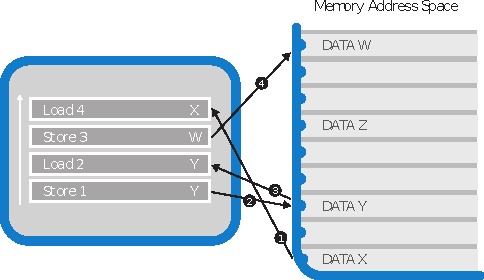
\includegraphics[width=0.6\textwidth]{methods/memory_disambiguation.pdf}
\caption{Beispiel für eine Speicher-Disambiguierung. Die Nummern in den Kreisen geben die chronologische Ausführungsreihenfolge an und der weiße Pfeil am linken Rand die Reihenfolge im Quellcode. Load 2 kann nicht früher ausgeführt werden, da er von Store 1 abhängig ist. Load 4 hingegen ist von den anderen Operationen unabhängig und kann daher vor Store 1 und Store 3 ausgeführt werden. Durch diese vorgezogene Ausführung können Instruktionen die den Wert von X benötigen im Folgenden von einer geringen Zugriffslatenz proftieren. \cite{CacheAssoWiki}.}
\end{figure}

\newtextend



\label{fig:colliding_addresses_js_measurement}
\begin{figure}[h]
\centering
\begin{scaletikzpicturetowidth}{\textwidth}
% Created by tikzDevice version 0.12 on 2018-09-13 19:52:01
% !TEX encoding = UTF-8 Unicode
\begin{tikzpicture}[scale=\tikzscale,y=21pt]
\definecolor{fillColor}{RGB}{255,255,255}
\path[use as bounding box,fill=fillColor,fill opacity=0.00] (0,0) rectangle (505.89,505.89);
\begin{scope}
\path[clip] ( 49.20, 61.20) rectangle (480.69,456.69);
\definecolor{drawColor}{RGB}{0,0,0}
\definecolor{fillColor}{RGB}{0,0,0}

\path[draw=drawColor,line width= 0.4pt,line join=round,line cap=round,fill=fillColor] ( 65.18,152.14) circle (  1.50);

\path[draw=drawColor,line width= 0.4pt,line join=round,line cap=round,fill=fillColor] ( 67.08,136.88) circle (  1.50);

\path[draw=drawColor,line width= 0.4pt,line join=round,line cap=round,fill=fillColor] ( 68.99,167.40) circle (  1.50);

\path[draw=drawColor,line width= 0.4pt,line join=round,line cap=round,fill=fillColor] ( 70.89,136.88) circle (  1.50);

\path[draw=drawColor,line width= 0.4pt,line join=round,line cap=round,fill=fillColor] ( 72.79,121.62) circle (  1.50);

\path[draw=drawColor,line width= 0.4pt,line join=round,line cap=round,fill=fillColor] ( 74.69,136.88) circle (  1.50);

\path[draw=drawColor,line width= 0.4pt,line join=round,line cap=round,fill=fillColor] ( 76.60,106.36) circle (  1.50);

\path[draw=drawColor,line width= 0.4pt,line join=round,line cap=round,fill=fillColor] ( 78.50,106.36) circle (  1.50);

\path[draw=drawColor,line width= 0.4pt,line join=round,line cap=round,fill=fillColor] ( 80.40,121.62) circle (  1.50);

\path[draw=drawColor,line width= 0.4pt,line join=round,line cap=round,fill=fillColor] ( 82.30,136.88) circle (  1.50);

\path[draw=drawColor,line width= 0.4pt,line join=round,line cap=round,fill=fillColor] ( 84.21,411.53) circle (  1.50);

\path[draw=drawColor,line width= 0.4pt,line join=round,line cap=round,fill=fillColor] ( 86.11,411.53) circle (  1.50);

\path[draw=drawColor,line width= 0.4pt,line join=round,line cap=round,fill=fillColor] ( 88.01,365.75) circle (  1.50);

\path[draw=drawColor,line width= 0.4pt,line join=round,line cap=round,fill=fillColor] ( 89.91,381.01) circle (  1.50);

\path[draw=drawColor,line width= 0.4pt,line join=round,line cap=round,fill=fillColor] ( 91.82,319.98) circle (  1.50);

\path[draw=drawColor,line width= 0.4pt,line join=round,line cap=round,fill=fillColor] ( 93.72,350.49) circle (  1.50);

\path[draw=drawColor,line width= 0.4pt,line join=round,line cap=round,fill=fillColor] ( 95.62,365.75) circle (  1.50);

\path[draw=drawColor,line width= 0.4pt,line join=round,line cap=round,fill=fillColor] ( 97.52,335.24) circle (  1.50);

\path[draw=drawColor,line width= 0.4pt,line join=round,line cap=round,fill=fillColor] ( 99.43,289.46) circle (  1.50);

\path[draw=drawColor,line width= 0.4pt,line join=round,line cap=round,fill=fillColor] (101.33,289.46) circle (  1.50);

\path[draw=drawColor,line width= 0.4pt,line join=round,line cap=round,fill=fillColor] (103.23,228.43) circle (  1.50);

\path[draw=drawColor,line width= 0.4pt,line join=round,line cap=round,fill=fillColor] (105.13,213.17) circle (  1.50);

\path[draw=drawColor,line width= 0.4pt,line join=round,line cap=round,fill=fillColor] (107.04,197.91) circle (  1.50);

\path[draw=drawColor,line width= 0.4pt,line join=round,line cap=round,fill=fillColor] (108.94,197.91) circle (  1.50);

\path[draw=drawColor,line width= 0.4pt,line join=round,line cap=round,fill=fillColor] (110.84,182.65) circle (  1.50);

\path[draw=drawColor,line width= 0.4pt,line join=round,line cap=round,fill=fillColor] (112.74,167.40) circle (  1.50);

\path[draw=drawColor,line width= 0.4pt,line join=round,line cap=round,fill=fillColor] (114.65,136.88) circle (  1.50);

\path[draw=drawColor,line width= 0.4pt,line join=round,line cap=round,fill=fillColor] (116.55,136.88) circle (  1.50);

\path[draw=drawColor,line width= 0.4pt,line join=round,line cap=round,fill=fillColor] (118.45,136.88) circle (  1.50);

\path[draw=drawColor,line width= 0.4pt,line join=round,line cap=round,fill=fillColor] (120.35,167.40) circle (  1.50);

\path[draw=drawColor,line width= 0.4pt,line join=round,line cap=round,fill=fillColor] (122.26,152.14) circle (  1.50);

\path[draw=drawColor,line width= 0.4pt,line join=round,line cap=round,fill=fillColor] (124.16,121.62) circle (  1.50);

\path[draw=drawColor,line width= 0.4pt,line join=round,line cap=round,fill=fillColor] (126.06, 91.11) circle (  1.50);

\path[draw=drawColor,line width= 0.4pt,line join=round,line cap=round,fill=fillColor] (127.96,106.36) circle (  1.50);

\path[draw=drawColor,line width= 0.4pt,line join=round,line cap=round,fill=fillColor] (129.87,121.62) circle (  1.50);

\path[draw=drawColor,line width= 0.4pt,line join=round,line cap=round,fill=fillColor] (131.77,121.62) circle (  1.50);

\path[draw=drawColor,line width= 0.4pt,line join=round,line cap=round,fill=fillColor] (133.67,106.36) circle (  1.50);

\path[draw=drawColor,line width= 0.4pt,line join=round,line cap=round,fill=fillColor] (135.57,167.40) circle (  1.50);

\path[draw=drawColor,line width= 0.4pt,line join=round,line cap=round,fill=fillColor] (137.48,152.14) circle (  1.50);

\path[draw=drawColor,line width= 0.4pt,line join=round,line cap=round,fill=fillColor] (139.38,121.62) circle (  1.50);

\path[draw=drawColor,line width= 0.4pt,line join=round,line cap=round,fill=fillColor] (141.28,136.88) circle (  1.50);

\path[draw=drawColor,line width= 0.4pt,line join=round,line cap=round,fill=fillColor] (143.18,136.88) circle (  1.50);

\path[draw=drawColor,line width= 0.4pt,line join=round,line cap=round,fill=fillColor] (145.09,121.62) circle (  1.50);

\path[draw=drawColor,line width= 0.4pt,line join=round,line cap=round,fill=fillColor] (146.99,106.36) circle (  1.50);

\path[draw=drawColor,line width= 0.4pt,line join=round,line cap=round,fill=fillColor] (148.89, 91.11) circle (  1.50);

\path[draw=drawColor,line width= 0.4pt,line join=round,line cap=round,fill=fillColor] (150.79,121.62) circle (  1.50);

\path[draw=drawColor,line width= 0.4pt,line join=round,line cap=round,fill=fillColor] (152.70,182.65) circle (  1.50);

\path[draw=drawColor,line width= 0.4pt,line join=round,line cap=round,fill=fillColor] (154.60,182.65) circle (  1.50);

\path[draw=drawColor,line width= 0.4pt,line join=round,line cap=round,fill=fillColor] (156.50,182.65) circle (  1.50);

\path[draw=drawColor,line width= 0.4pt,line join=round,line cap=round,fill=fillColor] (158.40,152.14) circle (  1.50);

\path[draw=drawColor,line width= 0.4pt,line join=round,line cap=round,fill=fillColor] (160.31,182.65) circle (  1.50);

\path[draw=drawColor,line width= 0.4pt,line join=round,line cap=round,fill=fillColor] (162.21,167.40) circle (  1.50);

\path[draw=drawColor,line width= 0.4pt,line join=round,line cap=round,fill=fillColor] (164.11,167.40) circle (  1.50);

\path[draw=drawColor,line width= 0.4pt,line join=round,line cap=round,fill=fillColor] (166.01,167.40) circle (  1.50);

\path[draw=drawColor,line width= 0.4pt,line join=round,line cap=round,fill=fillColor] (167.92,136.88) circle (  1.50);

\path[draw=drawColor,line width= 0.4pt,line join=round,line cap=round,fill=fillColor] (169.82,121.62) circle (  1.50);

\path[draw=drawColor,line width= 0.4pt,line join=round,line cap=round,fill=fillColor] (171.72,152.14) circle (  1.50);

\path[draw=drawColor,line width= 0.4pt,line join=round,line cap=round,fill=fillColor] (173.62,152.14) circle (  1.50);

\path[draw=drawColor,line width= 0.4pt,line join=round,line cap=round,fill=fillColor] (175.53,136.88) circle (  1.50);

\path[draw=drawColor,line width= 0.4pt,line join=round,line cap=round,fill=fillColor] (177.43,182.65) circle (  1.50);

\path[draw=drawColor,line width= 0.4pt,line join=round,line cap=round,fill=fillColor] (179.33,167.40) circle (  1.50);

\path[draw=drawColor,line width= 0.4pt,line join=round,line cap=round,fill=fillColor] (181.23,167.40) circle (  1.50);

\path[draw=drawColor,line width= 0.4pt,line join=round,line cap=round,fill=fillColor] (183.14,121.62) circle (  1.50);

\path[draw=drawColor,line width= 0.4pt,line join=round,line cap=round,fill=fillColor] (185.04,121.62) circle (  1.50);

\path[draw=drawColor,line width= 0.4pt,line join=round,line cap=round,fill=fillColor] (186.94,136.88) circle (  1.50);

\path[draw=drawColor,line width= 0.4pt,line join=round,line cap=round,fill=fillColor] (188.84,136.88) circle (  1.50);

\path[draw=drawColor,line width= 0.4pt,line join=round,line cap=round,fill=fillColor] (190.75,182.65) circle (  1.50);

\path[draw=drawColor,line width= 0.4pt,line join=round,line cap=round,fill=fillColor] (192.65,182.65) circle (  1.50);

\path[draw=drawColor,line width= 0.4pt,line join=round,line cap=round,fill=fillColor] (194.55,152.14) circle (  1.50);

\path[draw=drawColor,line width= 0.4pt,line join=round,line cap=round,fill=fillColor] (196.45,121.62) circle (  1.50);

\path[draw=drawColor,line width= 0.4pt,line join=round,line cap=round,fill=fillColor] (198.36,136.88) circle (  1.50);

\path[draw=drawColor,line width= 0.4pt,line join=round,line cap=round,fill=fillColor] (200.26,121.62) circle (  1.50);

\path[draw=drawColor,line width= 0.4pt,line join=round,line cap=round,fill=fillColor] (202.16, 75.85) circle (  1.50);

\path[draw=drawColor,line width= 0.4pt,line join=round,line cap=round,fill=fillColor] (204.06, 91.11) circle (  1.50);

\path[draw=drawColor,line width= 0.4pt,line join=round,line cap=round,fill=fillColor] (205.97,106.36) circle (  1.50);

\path[draw=drawColor,line width= 0.4pt,line join=round,line cap=round,fill=fillColor] (207.87, 91.11) circle (  1.50);

\path[draw=drawColor,line width= 0.4pt,line join=round,line cap=round,fill=fillColor] (209.77,152.14) circle (  1.50);

\path[draw=drawColor,line width= 0.4pt,line join=round,line cap=round,fill=fillColor] (211.67,152.14) circle (  1.50);

\path[draw=drawColor,line width= 0.4pt,line join=round,line cap=round,fill=fillColor] (213.58,152.14) circle (  1.50);

\path[draw=drawColor,line width= 0.4pt,line join=round,line cap=round,fill=fillColor] (215.48,152.14) circle (  1.50);

\path[draw=drawColor,line width= 0.4pt,line join=round,line cap=round,fill=fillColor] (217.38,121.62) circle (  1.50);

\path[draw=drawColor,line width= 0.4pt,line join=round,line cap=round,fill=fillColor] (219.28,152.14) circle (  1.50);

\path[draw=drawColor,line width= 0.4pt,line join=round,line cap=round,fill=fillColor] (221.19,396.27) circle (  1.50);

\path[draw=drawColor,line width= 0.4pt,line join=round,line cap=round,fill=fillColor] (223.09,365.75) circle (  1.50);

\path[draw=drawColor,line width= 0.4pt,line join=round,line cap=round,fill=fillColor] (224.99,365.75) circle (  1.50);

\path[draw=drawColor,line width= 0.4pt,line join=round,line cap=round,fill=fillColor] (226.89,396.27) circle (  1.50);

\path[draw=drawColor,line width= 0.4pt,line join=round,line cap=round,fill=fillColor] (228.80,350.49) circle (  1.50);

\path[draw=drawColor,line width= 0.4pt,line join=round,line cap=round,fill=fillColor] (230.70,350.49) circle (  1.50);

\path[draw=drawColor,line width= 0.4pt,line join=round,line cap=round,fill=fillColor] (232.60,396.27) circle (  1.50);

\path[draw=drawColor,line width= 0.4pt,line join=round,line cap=round,fill=fillColor] (234.50,335.24) circle (  1.50);

\path[draw=drawColor,line width= 0.4pt,line join=round,line cap=round,fill=fillColor] (236.41,335.24) circle (  1.50);

\path[draw=drawColor,line width= 0.4pt,line join=round,line cap=round,fill=fillColor] (238.31,274.20) circle (  1.50);

\path[draw=drawColor,line width= 0.4pt,line join=round,line cap=round,fill=fillColor] (240.21,197.91) circle (  1.50);

\path[draw=drawColor,line width= 0.4pt,line join=round,line cap=round,fill=fillColor] (242.11,243.69) circle (  1.50);

\path[draw=drawColor,line width= 0.4pt,line join=round,line cap=round,fill=fillColor] (244.02,228.43) circle (  1.50);

\path[draw=drawColor,line width= 0.4pt,line join=round,line cap=round,fill=fillColor] (245.92,228.43) circle (  1.50);

\path[draw=drawColor,line width= 0.4pt,line join=round,line cap=round,fill=fillColor] (247.82,228.43) circle (  1.50);

\path[draw=drawColor,line width= 0.4pt,line join=round,line cap=round,fill=fillColor] (249.72,167.40) circle (  1.50);

\path[draw=drawColor,line width= 0.4pt,line join=round,line cap=round,fill=fillColor] (251.63,182.65) circle (  1.50);

\path[draw=drawColor,line width= 0.4pt,line join=round,line cap=round,fill=fillColor] (253.53,182.65) circle (  1.50);

\path[draw=drawColor,line width= 0.4pt,line join=round,line cap=round,fill=fillColor] (255.43,136.88) circle (  1.50);

\path[draw=drawColor,line width= 0.4pt,line join=round,line cap=round,fill=fillColor] (257.33,136.88) circle (  1.50);

\path[draw=drawColor,line width= 0.4pt,line join=round,line cap=round,fill=fillColor] (259.24,167.40) circle (  1.50);

\path[draw=drawColor,line width= 0.4pt,line join=round,line cap=round,fill=fillColor] (261.14,136.88) circle (  1.50);

\path[draw=drawColor,line width= 0.4pt,line join=round,line cap=round,fill=fillColor] (263.04,228.43) circle (  1.50);

\path[draw=drawColor,line width= 0.4pt,line join=round,line cap=round,fill=fillColor] (264.94,136.88) circle (  1.50);

\path[draw=drawColor,line width= 0.4pt,line join=round,line cap=round,fill=fillColor] (266.85,152.14) circle (  1.50);

\path[draw=drawColor,line width= 0.4pt,line join=round,line cap=round,fill=fillColor] (268.75, 91.11) circle (  1.50);

\path[draw=drawColor,line width= 0.4pt,line join=round,line cap=round,fill=fillColor] (270.65,106.36) circle (  1.50);

\path[draw=drawColor,line width= 0.4pt,line join=round,line cap=round,fill=fillColor] (272.56,136.88) circle (  1.50);

\path[draw=drawColor,line width= 0.4pt,line join=round,line cap=round,fill=fillColor] (274.46,136.88) circle (  1.50);

\path[draw=drawColor,line width= 0.4pt,line join=round,line cap=round,fill=fillColor] (276.36,121.62) circle (  1.50);

\path[draw=drawColor,line width= 0.4pt,line join=round,line cap=round,fill=fillColor] (278.26,136.88) circle (  1.50);

\path[draw=drawColor,line width= 0.4pt,line join=round,line cap=round,fill=fillColor] (280.17,152.14) circle (  1.50);

\path[draw=drawColor,line width= 0.4pt,line join=round,line cap=round,fill=fillColor] (282.07,152.14) circle (  1.50);

\path[draw=drawColor,line width= 0.4pt,line join=round,line cap=round,fill=fillColor] (283.97,136.88) circle (  1.50);

\path[draw=drawColor,line width= 0.4pt,line join=round,line cap=round,fill=fillColor] (285.87,152.14) circle (  1.50);

\path[draw=drawColor,line width= 0.4pt,line join=round,line cap=round,fill=fillColor] (287.78,152.14) circle (  1.50);

\path[draw=drawColor,line width= 0.4pt,line join=round,line cap=round,fill=fillColor] (289.68,152.14) circle (  1.50);

\path[draw=drawColor,line width= 0.4pt,line join=round,line cap=round,fill=fillColor] (291.58,121.62) circle (  1.50);

\path[draw=drawColor,line width= 0.4pt,line join=round,line cap=round,fill=fillColor] (293.48,121.62) circle (  1.50);

\path[draw=drawColor,line width= 0.4pt,line join=round,line cap=round,fill=fillColor] (295.39, 91.11) circle (  1.50);

\path[draw=drawColor,line width= 0.4pt,line join=round,line cap=round,fill=fillColor] (297.29,106.36) circle (  1.50);

\path[draw=drawColor,line width= 0.4pt,line join=round,line cap=round,fill=fillColor] (299.19,152.14) circle (  1.50);

\path[draw=drawColor,line width= 0.4pt,line join=round,line cap=round,fill=fillColor] (301.09,106.36) circle (  1.50);

\path[draw=drawColor,line width= 0.4pt,line join=round,line cap=round,fill=fillColor] (303.00,136.88) circle (  1.50);

\path[draw=drawColor,line width= 0.4pt,line join=round,line cap=round,fill=fillColor] (304.90,136.88) circle (  1.50);

\path[draw=drawColor,line width= 0.4pt,line join=round,line cap=round,fill=fillColor] (306.80, 91.11) circle (  1.50);

\path[draw=drawColor,line width= 0.4pt,line join=round,line cap=round,fill=fillColor] (308.70,136.88) circle (  1.50);

\path[draw=drawColor,line width= 0.4pt,line join=round,line cap=round,fill=fillColor] (310.61,121.62) circle (  1.50);

\path[draw=drawColor,line width= 0.4pt,line join=round,line cap=round,fill=fillColor] (312.51,121.62) circle (  1.50);

\path[draw=drawColor,line width= 0.4pt,line join=round,line cap=round,fill=fillColor] (314.41,106.36) circle (  1.50);

\path[draw=drawColor,line width= 0.4pt,line join=round,line cap=round,fill=fillColor] (316.31,136.88) circle (  1.50);

\path[draw=drawColor,line width= 0.4pt,line join=round,line cap=round,fill=fillColor] (318.22,152.14) circle (  1.50);

\path[draw=drawColor,line width= 0.4pt,line join=round,line cap=round,fill=fillColor] (320.12,167.40) circle (  1.50);

\path[draw=drawColor,line width= 0.4pt,line join=round,line cap=round,fill=fillColor] (322.02,136.88) circle (  1.50);

\path[draw=drawColor,line width= 0.4pt,line join=round,line cap=round,fill=fillColor] (323.92,167.40) circle (  1.50);

\path[draw=drawColor,line width= 0.4pt,line join=round,line cap=round,fill=fillColor] (325.83,136.88) circle (  1.50);

\path[draw=drawColor,line width= 0.4pt,line join=round,line cap=round,fill=fillColor] (327.73,136.88) circle (  1.50);

\path[draw=drawColor,line width= 0.4pt,line join=round,line cap=round,fill=fillColor] (329.63,167.40) circle (  1.50);

\path[draw=drawColor,line width= 0.4pt,line join=round,line cap=round,fill=fillColor] (331.53,152.14) circle (  1.50);

\path[draw=drawColor,line width= 0.4pt,line join=round,line cap=round,fill=fillColor] (333.44,167.40) circle (  1.50);

\path[draw=drawColor,line width= 0.4pt,line join=round,line cap=round,fill=fillColor] (335.34,182.65) circle (  1.50);

\path[draw=drawColor,line width= 0.4pt,line join=round,line cap=round,fill=fillColor] (337.24,167.40) circle (  1.50);

\path[draw=drawColor,line width= 0.4pt,line join=round,line cap=round,fill=fillColor] (339.14,136.88) circle (  1.50);

\path[draw=drawColor,line width= 0.4pt,line join=round,line cap=round,fill=fillColor] (341.05, 91.11) circle (  1.50);

\path[draw=drawColor,line width= 0.4pt,line join=round,line cap=round,fill=fillColor] (342.95,106.36) circle (  1.50);

\path[draw=drawColor,line width= 0.4pt,line join=round,line cap=round,fill=fillColor] (344.85,121.62) circle (  1.50);

\path[draw=drawColor,line width= 0.4pt,line join=round,line cap=round,fill=fillColor] (346.75,152.14) circle (  1.50);

\path[draw=drawColor,line width= 0.4pt,line join=round,line cap=round,fill=fillColor] (348.66,152.14) circle (  1.50);

\path[draw=drawColor,line width= 0.4pt,line join=round,line cap=round,fill=fillColor] (350.56,197.91) circle (  1.50);

\path[draw=drawColor,line width= 0.4pt,line join=round,line cap=round,fill=fillColor] (352.46,182.65) circle (  1.50);

\path[draw=drawColor,line width= 0.4pt,line join=round,line cap=round,fill=fillColor] (354.36,182.65) circle (  1.50);

\path[draw=drawColor,line width= 0.4pt,line join=round,line cap=round,fill=fillColor] (356.27,197.91) circle (  1.50);

\path[draw=drawColor,line width= 0.4pt,line join=round,line cap=round,fill=fillColor] (358.17,197.91) circle (  1.50);

\path[draw=drawColor,line width= 0.4pt,line join=round,line cap=round,fill=fillColor] (360.07,167.40) circle (  1.50);

\path[draw=drawColor,line width= 0.4pt,line join=round,line cap=round,fill=fillColor] (361.97,197.91) circle (  1.50);

\path[draw=drawColor,line width= 0.4pt,line join=round,line cap=round,fill=fillColor] (363.88,152.14) circle (  1.50);

\path[draw=drawColor,line width= 0.4pt,line join=round,line cap=round,fill=fillColor] (365.78,197.91) circle (  1.50);

\path[draw=drawColor,line width= 0.4pt,line join=round,line cap=round,fill=fillColor] (367.68,197.91) circle (  1.50);

\path[draw=drawColor,line width= 0.4pt,line join=round,line cap=round,fill=fillColor] (369.58,152.14) circle (  1.50);

\path[draw=drawColor,line width= 0.4pt,line join=round,line cap=round,fill=fillColor] (371.49,197.91) circle (  1.50);

\path[draw=drawColor,line width= 0.4pt,line join=round,line cap=round,fill=fillColor] (373.39,197.91) circle (  1.50);

\path[draw=drawColor,line width= 0.4pt,line join=round,line cap=round,fill=fillColor] (375.29,182.65) circle (  1.50);

\path[draw=drawColor,line width= 0.4pt,line join=round,line cap=round,fill=fillColor] (377.19,182.65) circle (  1.50);

\path[draw=drawColor,line width= 0.4pt,line join=round,line cap=round,fill=fillColor] (379.10,167.40) circle (  1.50);

\path[draw=drawColor,line width= 0.4pt,line join=round,line cap=round,fill=fillColor] (381.00,136.88) circle (  1.50);

\path[draw=drawColor,line width= 0.4pt,line join=round,line cap=round,fill=fillColor] (382.90,136.88) circle (  1.50);

\path[draw=drawColor,line width= 0.4pt,line join=round,line cap=round,fill=fillColor] (384.80,152.14) circle (  1.50);

\path[draw=drawColor,line width= 0.4pt,line join=round,line cap=round,fill=fillColor] (386.71,167.40) circle (  1.50);

\path[draw=drawColor,line width= 0.4pt,line join=round,line cap=round,fill=fillColor] (388.61,167.40) circle (  1.50);

\path[draw=drawColor,line width= 0.4pt,line join=round,line cap=round,fill=fillColor] (390.51,167.40) circle (  1.50);

\path[draw=drawColor,line width= 0.4pt,line join=round,line cap=round,fill=fillColor] (392.41,136.88) circle (  1.50);

\path[draw=drawColor,line width= 0.4pt,line join=round,line cap=round,fill=fillColor] (394.32,167.40) circle (  1.50);

\path[draw=drawColor,line width= 0.4pt,line join=round,line cap=round,fill=fillColor] (396.22,136.88) circle (  1.50);

\path[draw=drawColor,line width= 0.4pt,line join=round,line cap=round,fill=fillColor] (398.12,136.88) circle (  1.50);

\path[draw=drawColor,line width= 0.4pt,line join=round,line cap=round,fill=fillColor] (400.02,182.65) circle (  1.50);

\path[draw=drawColor,line width= 0.4pt,line join=round,line cap=round,fill=fillColor] (401.93,182.65) circle (  1.50);

\path[draw=drawColor,line width= 0.4pt,line join=round,line cap=round,fill=fillColor] (403.83,197.91) circle (  1.50);

\path[draw=drawColor,line width= 0.4pt,line join=round,line cap=round,fill=fillColor] (405.73,197.91) circle (  1.50);

\path[draw=drawColor,line width= 0.4pt,line join=round,line cap=round,fill=fillColor] (407.63,182.65) circle (  1.50);

\path[draw=drawColor,line width= 0.4pt,line join=round,line cap=round,fill=fillColor] (409.54,197.91) circle (  1.50);

\path[draw=drawColor,line width= 0.4pt,line join=round,line cap=round,fill=fillColor] (411.44,197.91) circle (  1.50);

\path[draw=drawColor,line width= 0.4pt,line join=round,line cap=round,fill=fillColor] (413.34,167.40) circle (  1.50);

\path[draw=drawColor,line width= 0.4pt,line join=round,line cap=round,fill=fillColor] (415.24,121.62) circle (  1.50);

\path[draw=drawColor,line width= 0.4pt,line join=round,line cap=round,fill=fillColor] (417.15,121.62) circle (  1.50);

\path[draw=drawColor,line width= 0.4pt,line join=round,line cap=round,fill=fillColor] (419.05,182.65) circle (  1.50);

\path[draw=drawColor,line width= 0.4pt,line join=round,line cap=round,fill=fillColor] (420.95,167.40) circle (  1.50);

\path[draw=drawColor,line width= 0.4pt,line join=round,line cap=round,fill=fillColor] (422.85,136.88) circle (  1.50);

\path[draw=drawColor,line width= 0.4pt,line join=round,line cap=round,fill=fillColor] (424.76,106.36) circle (  1.50);

\path[draw=drawColor,line width= 0.4pt,line join=round,line cap=round,fill=fillColor] (426.66,381.01) circle (  1.50);

\path[draw=drawColor,line width= 0.4pt,line join=round,line cap=round,fill=fillColor] (428.56,396.27) circle (  1.50);

\path[draw=drawColor,line width= 0.4pt,line join=round,line cap=round,fill=fillColor] (430.46,365.75) circle (  1.50);

\path[draw=drawColor,line width= 0.4pt,line join=round,line cap=round,fill=fillColor] (432.37,396.27) circle (  1.50);

\path[draw=drawColor,line width= 0.4pt,line join=round,line cap=round,fill=fillColor] (434.27,365.75) circle (  1.50);

\path[draw=drawColor,line width= 0.4pt,line join=round,line cap=round,fill=fillColor] (436.17,396.27) circle (  1.50);

\path[draw=drawColor,line width= 0.4pt,line join=round,line cap=round,fill=fillColor] (438.07,396.27) circle (  1.50);

\path[draw=drawColor,line width= 0.4pt,line join=round,line cap=round,fill=fillColor] (439.98,442.04) circle (  1.50);

\path[draw=drawColor,line width= 0.4pt,line join=round,line cap=round,fill=fillColor] (441.88,335.24) circle (  1.50);

\path[draw=drawColor,line width= 0.4pt,line join=round,line cap=round,fill=fillColor] (443.78,274.20) circle (  1.50);

\path[draw=drawColor,line width= 0.4pt,line join=round,line cap=round,fill=fillColor] (445.68,289.46) circle (  1.50);

\path[draw=drawColor,line width= 0.4pt,line join=round,line cap=round,fill=fillColor] (447.59,258.95) circle (  1.50);

\path[draw=drawColor,line width= 0.4pt,line join=round,line cap=round,fill=fillColor] (449.49,213.17) circle (  1.50);

\path[draw=drawColor,line width= 0.4pt,line join=round,line cap=round,fill=fillColor] (451.39,213.17) circle (  1.50);

\path[draw=drawColor,line width= 0.4pt,line join=round,line cap=round,fill=fillColor] (453.29,182.65) circle (  1.50);

\path[draw=drawColor,line width= 0.4pt,line join=round,line cap=round,fill=fillColor] (455.20,167.40) circle (  1.50);

\path[draw=drawColor,line width= 0.4pt,line join=round,line cap=round,fill=fillColor] (457.10,182.65) circle (  1.50);

\path[draw=drawColor,line width= 0.4pt,line join=round,line cap=round,fill=fillColor] (459.00,167.40) circle (  1.50);

\path[draw=drawColor,line width= 0.4pt,line join=round,line cap=round,fill=fillColor] (460.90,152.14) circle (  1.50);

\path[draw=drawColor,line width= 0.4pt,line join=round,line cap=round,fill=fillColor] (462.81,167.40) circle (  1.50);

\path[draw=drawColor,line width= 0.4pt,line join=round,line cap=round,fill=fillColor] (464.71,167.40) circle (  1.50);
\end{scope}
\begin{scope}
\path[clip] (  0.00,  0.00) rectangle (505.89,505.89);
\definecolor{drawColor}{RGB}{0,0,0}

\path[draw=drawColor,line width= 0.4pt,line join=round,line cap=round] (112.74, 61.20) -- (398.12, 61.20);

\path[draw=drawColor,line width= 0.4pt,line join=round,line cap=round] (112.74, 61.20) -- (112.74, 55.20);

\path[draw=drawColor,line width= 0.4pt,line join=round,line cap=round] (207.87, 61.20) -- (207.87, 55.20);

\path[draw=drawColor,line width= 0.4pt,line join=round,line cap=round] (303.00, 61.20) -- (303.00, 55.20);

\path[draw=drawColor,line width= 0.4pt,line join=round,line cap=round] (398.12, 61.20) -- (398.12, 55.20);

\node[text=drawColor,anchor=base,inner sep=0pt, outer sep=0pt, scale=  1.00] at (112.74, 39.60) {3000};

\node[text=drawColor,anchor=base,inner sep=0pt, outer sep=0pt, scale=  1.00] at (207.87, 39.60) {3050};

\node[text=drawColor,anchor=base,inner sep=0pt, outer sep=0pt, scale=  1.00] at (303.00, 39.60) {3100};

\node[text=drawColor,anchor=base,inner sep=0pt, outer sep=0pt, scale=  1.00] at (398.12, 39.60) {3150};

\path[draw=drawColor,line width= 0.4pt,line join=round,line cap=round] ( 49.20,136.88) -- ( 49.20,442.04);

\path[draw=drawColor,line width= 0.4pt,line join=round,line cap=round] ( 49.20,136.88) -- ( 43.20,136.88);

\path[draw=drawColor,line width= 0.4pt,line join=round,line cap=round] ( 49.20,213.17) -- ( 43.20,213.17);

\path[draw=drawColor,line width= 0.4pt,line join=round,line cap=round] ( 49.20,289.46) -- ( 43.20,289.46);

\path[draw=drawColor,line width= 0.4pt,line join=round,line cap=round] ( 49.20,365.75) -- ( 43.20,365.75);

\path[draw=drawColor,line width= 0.4pt,line join=round,line cap=round] ( 49.20,442.04) -- ( 43.20,442.04);

\node[text=drawColor,rotate= 90.00,anchor=base,inner sep=0pt, outer sep=0pt, scale=  1.00] at ( 34.80,136.88) {30};

\node[text=drawColor,rotate= 90.00,anchor=base,inner sep=0pt, outer sep=0pt, scale=  1.00] at ( 34.80,213.17) {35};

\node[text=drawColor,rotate= 90.00,anchor=base,inner sep=0pt, outer sep=0pt, scale=  1.00] at ( 34.80,289.46) {40};

\node[text=drawColor,rotate= 90.00,anchor=base,inner sep=0pt, outer sep=0pt, scale=  1.00] at ( 34.80,365.75) {45};

\node[text=drawColor,rotate= 90.00,anchor=base,inner sep=0pt, outer sep=0pt, scale=  1.00] at ( 34.80,442.04) {50};

\path[draw=drawColor,line width= 0.4pt,line join=round,line cap=round] ( 49.20, 61.20) --
	(480.69, 61.20) --
	(480.69,456.69) --
	( 49.20,456.69) --
	( 49.20, 61.20);
\end{scope}
\begin{scope}
\path[clip] (  0.00,  0.00) rectangle (505.89,505.89);
\definecolor{drawColor}{RGB}{0,0,0}

\node[text=drawColor,anchor=base,inner sep=0pt, outer sep=0pt, scale=  1.00] at (264.94, 15.60) {4KiB block index};

\node[text=drawColor,rotate= 90.00,anchor=base,inner sep=0pt, outer sep=0pt, scale=  1.00] at ( 10.80,258.94) {SharedArrayBuffer timer value};
\end{scope}
\begin{scope}
\path[clip] ( 49.20, 61.20) rectangle (480.69,456.69);
\definecolor{drawColor}{RGB}{0,0,0}

\path[draw=drawColor,line width= 0.4pt,line join=round,line cap=round] ( 84.21,411.53) circle (  5.25);

\path[draw=drawColor,line width= 0.4pt,line join=round,line cap=round] (221.19,396.27) circle (  5.25);

\path[draw=drawColor,line width= 0.4pt,line join=round,line cap=round] (426.66,381.01) circle (  5.25);
\end{scope}
\end{tikzpicture}

\end{scaletikzpicturetowidth}
\caption{Erkennung von colliding addresses unter Javascript. Punkte geben die Latenz für eine Leseoperation auf eine fixe Adresse an, nachdem Schreiboperationen auf jeden der 64 Blöcke im aktuellen Fenster durchgeführt wurden.}
\end{figure}


TODO Algorithmus in Einzelheiten beschreiben
\todo[size=\footnotesize]{Beschreibe den Algorithmus bitte in einzelteilen, und gib auch den code dafür einzeln an. Der komplette Code gehört in den Anhang.}
%\todo[size=\footnotesize]{Nutze eine kleinere Schriftart für listings}


\section{Verdeckter Kanal}

Die maximale Sendegeschwindigkeit eines Kanals ist durch die Rate, mit welcher der Sender ein beliebiges Cache-Set primen kann, begrenzt.
Damit der Empfänger ein zufälliges Rauschen von einem Priming unterscheiden kann, sollte der Sender mehrere Einträge aus dem zu primenden Cache-Set verdrängen, wobei im Optimalfall die Anzahl der zugegriffenen Speicheradressen der Assoziativität des Caches entspricht.
Hiermit wird die Wahrscheinlichkeit erhöht, dass sich die vom Empfänger im Probe-Schritt gemessene Zugriffszeit signifikant von Fällen unterscheidet, in denen zufällig einzelne Einträge aus dem überwachten Cache-Set verdrängt werden. 
%Daraus folgernd nehmen wir an, dass der Sender in seiner Priming-Phase auf der Assoziativität entsprechend viele Speicheradressen zugreift.
Im Folgenden sollen verschiedene Methoden des Primens eines Cache-Sets verglichen werden, indem entweder die Anzahl der zugegriffen Speicheradressen oder die Zugriffsmethode verändert werden.
Wenn etwa die Zahl der zugegriffenen Speicheraddressen verringert wird, sind auf der einen Seite mehr Timeslots in einem Zeitabschnitt möglich, und die Chance sinkt, dass benachbarte Timeslots zusätzlich beeinflusst werden. Auf der anderen Seite sind die messbaren Ausschläge der Zugriffszeiten verringert, wodurch ein bewusst geprimtes Cache-Set schwieriger von einem Messrauschen oder von zufälligen Zugriffen unterschieden werden kann.
Sende- und Empfangsseite können durchaus abweichende Parameter verwenden, wenn wie etwa im vorliegenden Fall der Empfänger langsamer als der Sender arbeitet. Um die Timeslots anzugleichen, könnte der Empfänger die Dauer einer Priming-Operation durch die Senkung der Anzahl der zugegriffenen Speicheraddressen verringern und der Empfänger andersherum die Dauer für eine Priming-Operation erhöhen. 

\begin{algorithm}[h]
\DontPrintSemicolon
\caption{Pseudo-Code für Pointer-Chasing-Methode}
\label{alg:pointerChasing}

\Fn{$AccessTimeEvictionSet(pointerToAddress)$}{
    pointerToAddressFirst $\leftarrow$ pointerToAddress\;
    timestampBefore $\leftarrow$ getTimeStamp()\;
    \While{pointerToAddressFirst != pointerToAddress}{
        pointerToAddress $\leftarrow$ readValue(pointerToAddress)\;
    }
    \Return getTimeStamp() - timestampBefore
}

\end{algorithm}

Auf dem Testrechner benötigt ein in C geschriebenes Sendeprogramm für eine Million Prime-Vorgänge mit 16 Adressen und der Single-Pointer-Chasing-Methode (siehe Algorithmus \ref{alg:pointerChasing}) etwa 323 Millionen Taktzyklen.
Im Optimalfall kann im Timeslot $x$ ein durch den Sender erfolgter Prime-Vorgang als 1 und ein nicht erfolgter Prime-Vorgang  als 0 interpretiert werden.
%\todo{was ist ein erfolgreicher/nicht erfolgreicher prime-vorgang?}
%satz durch ergänzung vermutlich besser zu verstehen
Bei einem typischen All-Core-Turbo-Takt von 3,4 Ghz des i7-4770 ergibt sich so eine maximale Senderate von TODO ~10,5 Mbit/s.
Diese Rate wird jedoch vom Empfänger beschränkt, welcher zusätzlich noch eine Zeitmessung durchführen muss. Der Worst-Case ist hier eine in Webassembly geschriebene Empfangsroutine, da dort eine Zeitmessung kostenintensiver ist. In Chromium 66 können eine Million Messungen eines Cache-Sets in etwa 200 ms durchgeführt werden.
Im Mittel dauert eine Messung also 0,2 \textmu s, womit eine Empfangsrate von maximal ~5 MBit/s realisiert werden kann.

%Um die Performance zu erhöhen kann wie erwähnt die Anzahl der zugegriffen Speicheradressen reduziert werden. 
Im Folgenden soll die maximal mögliche Senderate unter optimalen Bedingungen ermittelt werden. 
Hierfür wird im Voraus ein Cache-Set ausgewählt, auf dem im Idle-Zustand des Systems ein geringes Rauschen herrscht.
Um die Synchronisation des Senders und Empfängers aufrechtzuerhalten, wird nach 10 gesendeten Bits ein Synchronisationsblock eingefügt, welcher durch $sb$-Prime-Vorgänge auf der Senderseite erzeugt wird. 
Eine 1 wird durch $s$-Prime-Vorgänge repräsentiert und eine 0 durch das Unterlassen der Prime-Vorgänge. 
Um die einzelnen Bits auseinanderzuhalten, wird zwischen jedem gesendeten Bit eine Pause von $p$-Taktzyklen eingelegt. \todo{vielleicht mal ein bild, mit dem ein konkreter btistring übertragen wird?}

%Um einen Kanal zu Initialisieren 


%TODO: benchmark cache set finder
%entwickle bessere benchmark prozedur, messe zeit für contract jedes es und mittle dann


%Problem: v8 compiliert lazy, d.h. nur häufig verwendete

\newtext




\newtextend

%Was wird angegriffen

%Verweis auf Paper Cache-Timing Attacks on RSA Key Generation